%% Rezolvari Electricitate si Magnetism %%

\section*{3. ELECTRICITATE ŞI MAGNETISM}
3.1. $E=E_{1}+E_{2}=7+7=14 \mathrm{~V} ; R_{e}=r_{1}+r_{1}+R=7 \Omega$;\\
$I=\frac{E}{R_{e}}=2 \mathrm{~A} ; E=R I^{2} t=1584 \mathrm{~J}$.\\
3.2. Rezistența conductorului este egală cu:\\
$R=\rho \frac{l}{S}=0,17 \Omega$, iar intensitatea curentului este $I=\frac{U_{c}}{R}=60 \mathrm{~A}$.\\
3.3. Noul circuit este reprezentat în Fig. prob. 3.3. Din legile lui Kirchhoff:

$$
\left.\begin{array}{l}
I_{3}=I_{1}+I_{2} \\
R_{1} I_{1}=R_{2} I_{2} \\
E=R_{3} I_{3}+R_{2} I_{2}
\end{array}\right\} \Rightarrow I_{1}=\frac{R_{2} E}{R_{1} R_{2}+R_{1} R_{3}+R_{2} R_{3}}=1 \mathrm{~A}
$$

\begin{center}
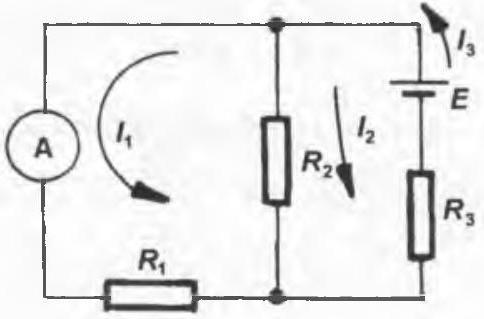
\includegraphics[max width=\textwidth]{2025_07_01_5b3ff9fa0d508c8e9f17g-341(1)}
\end{center}

Fig. prob. 3.3\\
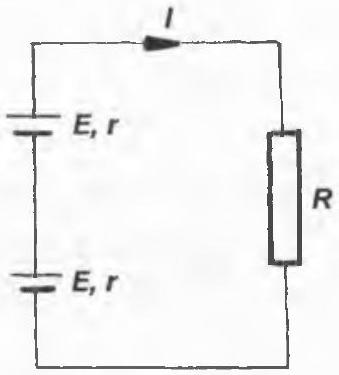
\includegraphics[max width=\textwidth, center]{2025_07_01_5b3ff9fa0d508c8e9f17g-341(2)}

Fig. prob. 3.4\\
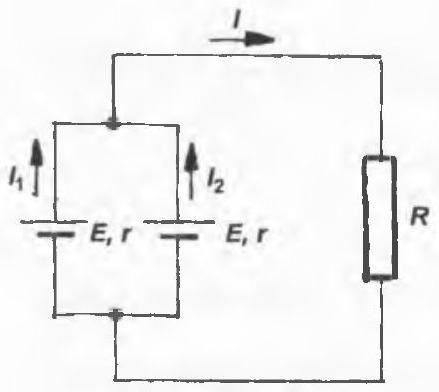
\includegraphics[max width=\textwidth, center]{2025_07_01_5b3ff9fa0d508c8e9f17g-341}

Fig. prob. 3.5\\
3.4. Din legea lui Ohm (Fig. prob. 3.4): $I=\frac{2 E}{R+2 r}=2 \mathrm{~A}$.\\
3.5. Din legile lui Kirchhoff (Fig. prob. 3.5)

$$
\left.\begin{array}{l}
I=I_{1}+I_{2} \\
E:=r I_{2}+R I \\
E=r I_{1}+R I
\end{array}\right\} \Rightarrow I_{1}=I_{2}=\frac{E}{r+2 R}=0,5 \mathrm{~A}
$$

sau din legea lui Ohm,

$$
r_{e}=\frac{r}{2} ; I=\frac{E}{R+\frac{r}{2}}=1 \mathrm{~A}
$$

şi $\quad I_{1}=I_{2}=\frac{I}{2}=0,5 \mathrm{~A}$.\\
3.6. Din egalitatea puterilor $R_{1} \frac{E^{2}}{\left(r+R_{1}\right)^{2}}=R_{2} \frac{E^{2}}{\left(r+R_{2}\right)^{2}}$ rezultă:

$$
r=\sqrt{R_{1} R_{2}}=20 \Omega
$$

3.7. La conectarea primului rezistor, $W=\frac{U^{2}}{R_{1}} t_{1}$, iar $t_{1}=\frac{W}{U^{2}} R_{1}$. La conectarea celui de-al doilea rezistor, $W=\frac{U^{2}}{R_{2}} t_{2}$, iar $t_{2}=\frac{W}{U^{2}} R_{2}$. Dacă se conectează ambele rezistoare în paralel, $W=\left(\frac{1}{R_{1}}+\frac{1}{R_{2}}\right) U^{2} t$, de unde:

$$
t=\frac{W}{U^{2}} \cdot \frac{R_{1} R_{2}}{R_{1}+R_{2}}=\frac{\frac{W}{U^{2}} R_{1} \cdot \frac{W}{U^{2}} R_{2}}{\frac{W}{U^{2}} R_{1}+\frac{W}{U^{2}} R_{2}}=\frac{t_{1} t_{2}}{t_{1}+t_{2}}=12 \mathrm{~s}
$$

3.8. Din expresia puterii, $P=P_{b}+P_{r}=\frac{U^{2}}{R_{b}}+R_{r} I^{2}$ sau $P=\left(R_{b}+R_{r}\right) I^{2}$, de unde $R_{b}=\frac{P}{I^{2}}-R_{r}$, rezultă ecuația în $I: R_{r}^{2} I^{4}-\left(2 R_{r} P+U^{2}\right) I^{2}+P=0$. Astfel, $I^{2}=\frac{2 R_{r} P+U^{2} \pm U \sqrt{4 P R_{r}+U^{2}}}{2 R_{r}^{2}}=\left\{\begin{array}{l}4 \mathrm{~A}^{2} \\ 25 \mathrm{~A}^{2}\end{array}\right.$, de unde $I=\left\{\begin{array}{l}2 \mathrm{~A} \\ 5 \mathrm{~A}\end{array}\right.$.

Observăm că $P_{r}=R_{r} I^{2}=500 \mathrm{~W}$, valoare ce nu corespunde enunțului problemei. Deci, $I=5 \mathrm{~A}$ nu este o soluție, deoarece becul şi reostatul consumă împreună 200 W .\\
3.9. Din legea electrolizei $m=K I t$, unde $m=\rho_{\mathrm{Ni}} S d$, astfel că $\rho_{\mathrm{Ni}} S d=K_{\mathrm{Ni}} I t$, iar $t=\frac{\rho_{\mathrm{Ni}} S d}{K_{\mathrm{Ni}} I}=22 \mathrm{~s}$.\\
3.10. Din legea lui Ohm $I=\frac{E}{R+r}$ şi a lui Joule - Lenz rezultă $P=I^{2} R=\frac{E^{2} R}{(R+r)^{2}}=P(R)$. Condiția de maxim a puterii se scrie: $\frac{\mathrm{d} P(R)}{\mathrm{d} R}=0$, adică $E^{2} \frac{(R+r)^{2}-2(R+r) R}{(R+r)^{4}}=0$, de unde $R=r ; R=-r$ (nu are sens fizic).

Deci, $U=I r=\frac{E}{2 r} r=1 \mathrm{~V}$.\\
3.11. Din condițiile $\left\{\begin{array}{l}R_{1}+R_{2}+R_{3}=R_{s}=9 \\ \frac{1}{R_{p}}=\frac{1}{R_{1}}+\frac{1}{R_{2}}+\frac{1}{R_{3}}=\frac{13}{12} \text { rezultă }\end{array}\right.$ $\left\{\begin{array}{l}R+R+R_{0}+R-R_{0}=9 \\ \frac{1}{R}+\frac{1}{R+R_{0}}+\frac{1}{R-R_{0}}=\frac{13}{12}\end{array}\right.$, de unde $3 R=9$, iar $R=3 \Omega$.\\
Astfel: $R_{0}=R \sqrt{\frac{R-3 R_{p}}{R-R_{p}}}=1 \Omega$ şi $R_{1}=3 \Omega, R_{2}=4 \Omega, R_{3}=2 \Omega$.\\
3.12. $R_{s}=n R ; R_{p}=R / n \Rightarrow R_{s} / R_{p}=n^{2}$.\\
3.13. Când funcționează doar primul rezistor $Q=\frac{U^{2}}{R_{1}} t_{1}$, iar pentru al doilea $Q=\frac{U^{2}}{R_{2}} t_{2}$. Dacă se leagă cele două rezistoare în serie $Q=\frac{U^{2}}{R_{1}+R_{2}} t$. Dar $R_{1}=\frac{U^{2} t_{1}}{Q} ; R_{2}=\frac{U^{2} t_{2}}{Q}$, astfel încât $Q=\frac{U^{2} t Q}{U^{2} t_{1}+U^{2} t_{2}}$, de unde $t=t_{1}+t_{2}$.\\
3.14. $\eta_{1}=\frac{R}{R+r_{1}} ; \eta_{2}=\frac{R}{R+r_{2}} ; \eta=\frac{R}{R+\left(r_{1}+r_{2}\right)}$;

$$
r_{1}=\frac{R\left(1-\eta_{1}\right)}{\eta_{1}} ; r_{2}=\frac{R\left(1-\eta_{2}\right)}{\eta_{2}} \Rightarrow \eta=\frac{R}{R+R\left(\frac{1-\eta_{1}}{\eta_{1}}+\frac{1-\eta_{2}}{\eta_{2}}\right)} \Rightarrow
$$

$$
\eta=\frac{\eta_{1} \eta_{2}}{\eta_{1}+\eta_{2}-\eta_{1} \eta_{2}}
$$

3.15. Din expresia $I=n e S v$ rezultă $v=\frac{I}{n e S}=\frac{U}{n e S R}$. Astfel $v^{\prime}=\frac{2 U}{n e S R}$ şi $\frac{v^{\prime}}{v}=2$, adică viteza electronilor creşte de 2 ori.\\

3.16. Conform definiției: $I=\frac{e}{T}=e \cdot v=9,6 \cdot 10^{-4} \mathrm{~A}$.\\

3.17. $I=n e S v$ rezultă $v=\frac{I}{n e S}=\frac{U}{n e S R}=\frac{U}{n e S \frac{\rho l}{S}}=\frac{U}{n e \rho l}$. Deoarece viteza de transport a electronilor este independentă de diametrul conductorului rezultă că în experiența considerată viteza va rămâne constantă.\\

3.18. Conform circuitului din Fig. prob. 3.18,\\ $E_{1}+E_{2}=I_{1} r_{1}+I_{2}\left(R+r_{2}\right)$\\ $E_{3}+E_{2}=I_{3} r_{3}+I_{2}\left(R+r_{2}\right)$\\ şi $\quad I_{2}=I_{1}+I_{3}$, de unde\\ $I_{2}=\frac{\left(E_{1}+E_{2}\right) r_{3}+\left(E_{2}+E_{3}\right) r_{1}}{r_{1} r_{3}+\left(R+r_{2}\right)\left(r_{1}+r_{3}\right)}=\frac{27}{203} \mathrm{~A}$\\ iar\\ $U_{\mathrm{AB}}=V_{\mathrm{B}}-V_{\mathrm{A}}=I_{2}\left(R+r_{2}\right)-E_{2}=-9 \mathrm{~V}$.\\ \begin{center} 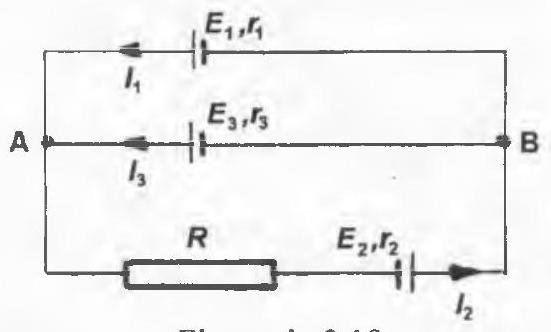
\includegraphics[max width=\textwidth]{2025_07_01_5b3ff9fa0d508c8e9f17g-344}\\ Fig. prob. 3.18 \end{center}\\

3.19. Prin bec trebuie să circule un curent de intensitate $I=\frac{P}{U}=0,5 \mathrm{~A}$. Becul are rezistența electrică $R_{\mathrm{b}}=\frac{U}{I}=240 \Omega$. Scriind legea lui Ohm pentru circuitul cu rezistența adițională, $U_{1}=I\left(R_{\mathrm{a}}+R_{\mathrm{b}}\right)$, rezultă că $R_{\mathrm{a}}=\frac{U_{1}}{I}-R_{\mathrm{b}}=200 \Omega$.\\

3.20. Din legile lui Kirchhoff: $I=I_{1}+I_{2}, \quad E_{1}-E_{2}=I_{1} r_{1}-I_{2} r_{2} \quad$ şi $E_{2}=I_{2} r_{2}+I R$, rezultă că: $I=\frac{\frac{E_{1}}{r_{1}}+\frac{E_{2}}{r_{2}}}{1+R\left(\frac{1}{r_{1}}+\frac{1}{r_{2}}\right)}$,\\ iar tensiunea $U=I R=\frac{\frac{E_{1}}{r_{1}}+\frac{E_{2}}{r_{2}}}{\frac{1}{R}+\frac{1}{r_{1}}+\frac{1}{r_{2}}}=7,33 \mathrm{~V}$.\\

3.21. Rezistenţa firelor de legătură este $R_{f}=\rho \frac{2 d}{S}$, cu condiția ca $\eta P=I^{2} R_{f}$, de unde $I=\sqrt{\frac{\eta P}{R_{f}}}$, iar $I U=(1-\eta) P$, de unde:\\ $U=(1-\eta) \sqrt{\frac{R_{f} P}{\eta}}=73,4 \mathrm{kV}$.\\

3.22. Conform circuitului din Fig. prob. 3.22, $I=I_{1}+I_{2} ; \quad I_{1} R_{1}-I_{2} R_{2}=0$,\\ unde, $\quad \frac{R_{1}}{R_{2}}=\frac{l_{1}}{l_{2}}=\frac{1}{3}$, iar $R_{1}+R_{2}=R$.\\ Astfel,\\ $I_{1}=I \frac{R_{2}}{R_{1}+R_{2}}=I \frac{1}{1+\frac{R_{1}}{R_{2}}}=\frac{3}{4} I$\\ şi\\ $U_{\mathrm{AB}}=I_{1} R_{1}=\frac{3}{4} I \cdot \frac{R}{4}=6 \mathrm{~V}$.\\ \begin{center} 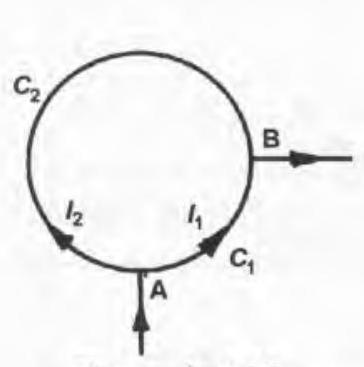
\includegraphics[max width=\textwidth, center]{2025_07_01_5b3ff9fa0d508c8e9f17g-345}\\ Fig. prob. 3.22 \end{center}\\

3.23. Fără rezistență adițională voltmetrul poate măsura o tensiune $U_{0}=i_{0} R_{0}$. Pentru a măsura o tensiune $U$ are nevoie de rezistența adițională:\\ $r_{a}=\frac{U-U_{0}}{i_{0}}=r_{0}\left(\frac{U}{U_{0}}-1\right)=r_{0}\left(\frac{U}{i_{0} r_{0}}-1\right)=290,2 \Omega$.\\

3.24. Puterea debitată de sursă în exterior este egală cu:\\ $P=I^{2} R=\left(\frac{n E}{R+n r}\right)^{2} R$,\\ a cărei valoare maximă se obține din condiția:\\ $\frac{\mathrm{d} P}{\mathrm{~d} R}=\frac{n^{2} E^{2}(R+n r)^{2}-2 n^{2} E^{2} R(R+n r)}{(R+n r)^{4}}=0$\\ de unde $R=n r$. Deci, $P_{\max }=n \frac{E^{2}}{4 r}=8,16 \mathrm{~W}$.\\

3.25. Rezistorul $R_{1}$ este confectionat pentru un curent electric $I_{1}=\sqrt{\frac{P_{1}}{R_{1}}}=10^{-2} \mathrm{~A}$, iar rezistorul $R_{2}$ pentru un curent $I_{2}=\sqrt{\frac{P_{2}}{R_{2}}}=2 \cdot 10^{-2} \mathrm{~A}$. Pentru ca să funcționeze în condiții optime alegem curentul $I_{1}$ şi atunci $U=I_{1}\left(R_{1}+R_{2}\right)=500 \mathrm{~V}$.\\

3.26. $I_{1}=\frac{E}{R+n r}$ şi $I_{2}=\frac{E}{2 \cdot\left(R+\frac{n}{2} r\right)}$, de unde $n=\frac{2 E}{r}\left(\frac{1}{I_{1}}-\frac{1}{2 I_{2}}\right)=20$.\\

3.27. Dacă se leagă circuitele în serie, acestea nu vor fi independente, iar dacă se leagă în paralel, rezistentele fiind diferite, nu se poate asigura aceeaşi valoare pentru curentul electric. Circuitele vor fi legate ca în Fig. prob. 3.27. Astfel,\\ $n_{1} E=2 I n_{1} r+I R_{1}$\\ $\left(n_{2}-n_{1}\right) E=I\left[\left(n_{2}-n_{1}\right) \cdot r-R_{1}+R_{2}\right]$\\ de unde $n_{1}=4$ şi $n_{2} \cong 13$.\\ \begin{center} 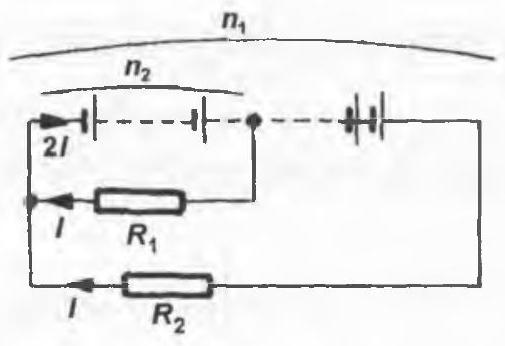
\includegraphics[max width=\textwidth, center]{2025_07_01_5b3ff9fa0d508c8e9f17g-346}\\ Fig. prob. 3.27 \end{center}\\

3.28. Când în circuit este legat doar becul: $P_{1}=\frac{U_{1}^{2}}{R_{1}}$, unde $U_{1}=I R_{1}=\frac{U R_{1}}{R_{1}+R_{2}}$, adică $U_{1}^{2}-U U_{1}+P R_{1}=0$, de unde $U_{1}=210 \mathrm{~V}$ şi $R_{1}=441 \Omega$. În al doilea caz, $P_{2}=\frac{U_{2}^{2}}{R_{2}}$, unde\\ $U_{2}=I^{\prime} \frac{R_{1} R_{2}}{R_{1}+R_{2}}=\frac{U}{\frac{R_{1} R_{2}}{R_{1}+R_{2}}+R} \cdot \frac{R_{1} R_{2}}{R_{1}+R_{2}}$\\ de unde $U_{2}^{2}\left(R+R_{1}\right)-U U_{2} R_{1}+R R_{1} P_{2}=0$, din care $U_{2}=160 \mathrm{~V}$ şi $R_{2}=64 \Omega$. Deci, $U_{2}-U_{1}=-50 \mathrm{~V}$.\\

3.29. Conform circuitului din Fig. prob. 3.29., datorită simetriei:\\ $I=I_{1}+I_{2}, \quad I_{2}=I_{1}+I_{3}, \quad I_{1} R-I_{2} R=I_{3} R=0$\\ de unde $I_{3}=0, \quad I_{1}=I_{2}=\frac{I}{2}$, iar $R_{e}=\frac{U_{A B}}{I}=\frac{2 I_{2} R+I_{3} R}{I}=R$.\\ \begin{center} 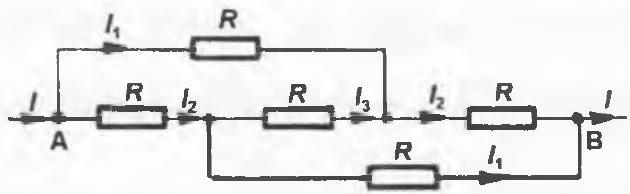
\includegraphics[max width=\textwidth, center]{2025_07_01_5b3ff9fa0d508c8e9f17g-347(1)}\\ Fig. prob. 3.29 \end{center}\\

3.30. Conform circuitului din Fig. prob. 3.30, $E_{1}-E_{2}=I_{1} r_{1}-I_{2} r_{2}$, iar $E_{2}=I_{2} r_{2}+\left(I_{1}+I_{2}\right) R$, de unde\\ $I_{2}=\frac{I_{1} r_{1}-E_{1}+E_{2}}{r_{2}}=\frac{E_{2}-I_{1} R}{r_{2}+R}$, iar $I_{1}=\frac{E_{1}\left(r_{2}+R\right)-E_{2} R}{r_{1}\left(r_{2}+R\right)}=0 $.\\ Astfel, $E_{1}=\frac{E_{2} R}{r_{2}+R}=113,6 \mathrm{~V}$.\\ \begin{center} 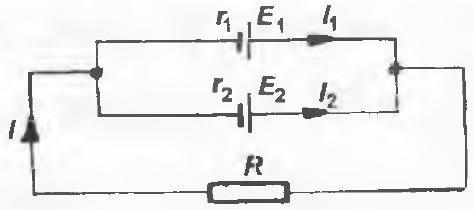
\includegraphics[max width=\textwidth, center]{2025_07_01_5b3ff9fa0d508c8e9f17g-347}\\ Fig. prob. 3.30 \end{center}\\

3.31. În primul caz (Fig. prob. 3.31 a ): $V_{1}=\eta_{V} \cdot I=\eta_{V} \cdot \frac{E}{\eta_{V}+r}$.\\ În al doilea caz (Fig. prob. 3.31 b):\\ $\frac{1}{r_{\text {echiv }}}=\frac{1}{r_{V}}+\frac{1}{r_{V}}=\frac{2}{r_{V}}$, iar $V_{1}=r_{V} \cdot I=r_{V} \cdot \frac{E}{r_{V}+r}$, si $V_{2}=\frac{r_{V}}{2} \cdot \frac{E}{\frac{r_{V}}{2}+r}=\frac{E \cdot r_{V}}{r_{V}+2 r}$\\ de unde $E=\frac{V_{1} r_{V}+V_{1} r}{r_{V}}$ şi $r=\frac{E r_{V}-V_{1} r_{V}}{V_{1}}$. Astfel, $E=\frac{V_{1} V_{2}}{2 V_{2}-V_{1}}$.\\ \begin{center} 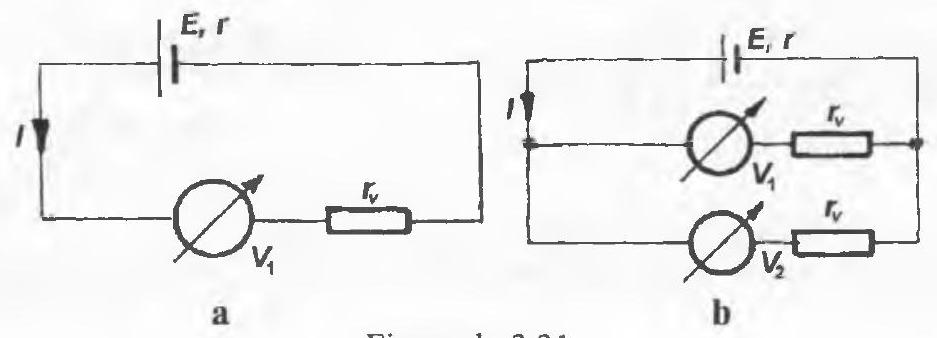
\includegraphics[max width=\textwidth, center]{2025_07_01_5b3ff9fa0d508c8e9f17g-347(2)}\\ Fig. prob. 3.31 \end{center}\\

3.32. Din legea lui Ohm,\\ $I=\frac{E}{\frac{R_{1} R_{2}}{R_{1}+R_{2}}}=\frac{E\left(R_{1}+R_{2}\right)}{R_{1} R_{2}}=3 \mathrm{~A}$.\\ Din legea lui Kirchhoff, $E=R_{1} I_{1}$, rezultă $I_{1}=\frac{E}{R_{1}}=2 \mathrm{~A}$. Asemănător,\\ $I_{2}=I-I_{1}=1 \mathrm{~A}$.\\ Deci $I=3 \mathrm{~A} ; I_{1}=2 \mathrm{~A} ; I_{2}=1 \mathrm{~A}$.\\

3.33. Rezistența liniei bifilare este: $R=\rho \frac{2 l}{S}=\frac{8 l \rho}{\pi D^{2}}$, iar intensitatea curentului, $I=\frac{U^{\prime}}{\rho \frac{2 l}{S}}=\frac{P}{U-U^{\prime}}$, astfel că $D=\sqrt{\frac{4 P \cdot \rho \cdot 2 l}{\pi\left(U U^{\prime}-U^{\prime 2}\right)}}=\frac{2 \cdot 10^{-2}}{\sqrt{\pi}} \mathrm{~m}$.\\

3.34. Rezistența echivalentă a circuitului:\\ $R_{c}=R_{3}+R_{12}+R_{4}=R_{3}+\frac{R_{1} R_{2}}{R_{1}+R_{2}}+R_{4}=3,8 \Omega$\\ iar $I=\frac{E}{R_{c}+r}=6 \mathrm{~A}$.\\ Din ecuațiile Kirchhoff scrise pentru nodul C şi ochiul 1 rezultă:\\ $I_{1}=I \cdot \frac{R_{2}}{R_{1}+R_{2}}=3,6 \mathrm{~A}$ şi $I_{2}=I \cdot \frac{R_{1}}{R_{1}+R_{2}}=2,4 \mathrm{~A}$\\

3.35. Rezistența echivalentă,\\ $R_{e}=R+\frac{R_{1} R_{2}}{R_{1}+R_{2}}=6 \Omega$\\ iar intensitatea curentului $I=\frac{E}{R_{e}}=3 \mathrm{~A}$. Din legile lui Kirchhoff, $I=I_{1}+I_{2}$ şi $I_{1} R_{1}=I_{2} R_{2} \quad$ rezultă $\quad I_{1}+I_{2}=3 \quad$ şi $\quad 6 I_{1}=3 I_{2}$, de unde $\quad I_{2}=2 I_{1} \quad$ și $I_{1}=1 \mathrm{~A}, I_{2}=2 \mathrm{~A}$.\\

3.36. Schema echivalentă montajului este cea din Fig. prob. 3.36. Avem:\\ $R_{e}=\frac{2 R \cdot 2 R}{2 R+2 R}=R$\\ \begin{center} 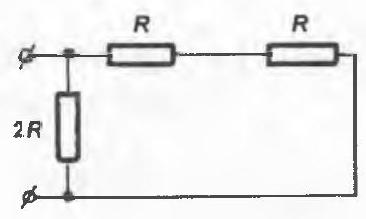
\includegraphics[max width=\textwidth]{2025_07_01_5b3ff9fa0d508c8e9f17g-348}\\ Fig. prob. 3.36 \end{center}\\

3.37. Puterea debitată de o sursă pe o rezistență exterioară este $P=E^{2} \cdot \frac{R}{(R+r)^{2}}$.\\ Valoarea maximă se obține atunci când $R=r, \operatorname{iar} P_{\max }=\frac{E^{2}}{4 r}$.\\ Din ecuația $P=f P_{\max }$ rezultă $\frac{R}{(R+r)^{2}}=\frac{f}{4 r}$, de unde\\ $R_{1,2}=r \cdot \frac{2-f \pm 2 \sqrt{1-f}}{f}$.\\ Astfel, raportul tensiunilor devine:\\ $\frac{U_{1}}{U_{2}}=\frac{I_{1} R_{1}}{I_{2} R_{2}}=\frac{E R_{1}}{R_{1}+r} \cdot \frac{R_{2}+r}{E R_{2}}=\frac{R_{1} R_{2}+R_{1 r}}{R_{1} R_{2}+R_{2 r}} .$\\ Efectuând calculele, se obține:\\ $\frac{U_{1}}{U_{2}}=\frac{1+\sqrt{1-f}}{1-\sqrt{1-f}}=6,54$.\\

3.38. Fie $I_{0}$ curentul ce trece prin cele $(n-1)$ pile legate la fel. Atunci $I=(n-1) I_{0}$. Aplicând legea a II-a a lui Kirchhoff pe un ochi format din latura ce conține pila legată în opoziție şi o latură arbitrară, avem $E+E=I_{0} r+I r$ de unde $I_{0}=\frac{2 E}{r}-I$. Rezultă $I=(n-1)\left(\frac{2 E}{r}-I\right)=\frac{n-1}{n} \cdot \frac{2 E}{r}$.\\

3.39. La $t=0^{\circ} \mathrm{C}$ avem $I_{0}=\frac{U}{R_{0}}$, iar la temperatura $t=100^{\circ} \mathrm{C}$ :\\ $I=\frac{U}{R(t)}=\frac{U}{R_{0}(1+\alpha \cdot t)}=\frac{I_{0}}{(1+\alpha \cdot t)}$.\\ Rezultǎ $\alpha=\frac{I_{0}-I}{I \cdot t}=\frac{I_{0}-I}{I \cdot t}=4 \cdot 10^{-3} \mathrm{grad}^{-1}$.\\

3.40. La legarea în serie $I=\frac{E}{R_{1}+R_{2}+r}$, iar la legarea în paralel $I^{\prime}=\frac{E}{\frac{R_{1} R_{2}}{R_{1}+R_{2}}+r}$. Deoarece $I^{\prime}=3 I$ găsim $r=\frac{R_{1}^{2}+R_{2}^{2}-R_{1} R_{2}}{2\left(R_{1}+R_{2}\right)}=1,4 \Omega$.\\

3.41. La legarea in paralel $I_{1}=\frac{E}{R+\frac{r}{2}}=\frac{2 E}{2 R+r}$, iar la legarea în serie $I_{2}=\frac{2 E}{R+2 r}$. Deoarece $I_{2}=1,7 I_{1}$, găsim $r=2 \Omega$.\\

3.42. $W=P t=0,18 \mathrm{~kWh}$. Costul energiei va fi $0,18 \cdot 1300=234 \mathrm{~lei}$.\\

3.43. $I=\frac{N e}{t}, \operatorname{deci} N=\frac{I t}{e}=24 \cdot 10^{19}$ electroni.\\

3.44. Din $\frac{E}{R+r}=\frac{1}{29} \cdot \frac{E}{r}$ rezultă $r=\frac{R}{28}=50 \Omega$.\\

3.45. $R=\frac{U^{2}}{50 P}=2,7 \Omega$.\\

3.46. $R=\frac{\left(R_{1}+R_{2}\right)\left(R_{2}+R_{4}\right)}{R_{1}+R_{2}+R_{2}+R_{4}}=\frac{21}{10} \Omega$, iar $R^{\prime}=\frac{R_{1} R_{3}}{R_{1}+R_{3}}+\frac{R_{2} R_{4}}{R_{2}+R_{4}}=\frac{25}{12}$. Deci $\frac{R}{R^{\prime}}=\frac{126}{125}$.\\

3.47. Curentul de scurtcircuit este $I_{S c}=\frac{E}{r}$, iar $U=E-I r=\frac{E R}{R+\frac{E}{I_{S c}}}$. Deci\\ $R=\frac{E U}{(E-U) I_{s c}}=4,4 \Omega$\\

3.48. Randamentul reprezintă raportul dintre puterea utilă (debitată pe circuitul exterior sursei) şi puterea totală debitată de sursă\\ $\eta=\frac{P_{u}}{P_{c}}=\frac{R I^{2}}{(R+r) I^{2}}=\frac{R}{R+r}$\\ unde $R$ este rezistența electrică a firului, $R=\rho \frac{l}{S}$, de unde $\eta=92 \%$.\\

3.49. Răspuns corect: B).\\

3.50. Aplicând teoremele lui Kirchhoff şi punând condiția ca intensitatea curentului care circulă prin rezistorul de rezistență $R$ să fie nulă se obține:\\ $\frac{E_{1}}{r_{1}}=\frac{E_{2}}{r_{2}}$\\

3.51. Din legea lui Ohm, $I=\frac{U}{R}=\frac{U}{\rho \frac{l}{S}}=50 \mathrm{~A}$.\\

3.52. Conform legilor lui Joule-Lenz şi a lui Ohm:\\ $P=I_{1}^{2} R_{1}$, unde $I_{1}=\frac{E}{R_{1}+r}$, iar\\ $P=I_{2}^{2} R_{2}$, unde $I_{2}=\frac{E}{R_{2}+r}$.\\ Din egalitatea puterilor rezultă:\\ $r=\sqrt{R_{1} R_{2}}=14 \Omega$\\

3.53. $E=i_{1} r_{1}+I R=i_{2} r_{2}+I R, i_{1} r_{1}=i_{2} r_{2}, \quad i_{2}=\frac{i_{1} r_{1}}{r_{2}}$,\\ $I=i_{1}+i_{2}=i_{1}\left(1+\frac{r_{1}}{r_{2}}\right), \quad R=\frac{E-i_{1} \eta_{1}}{I}=\frac{E-i_{1} \eta_{1}}{i_{1} \cdot \frac{\eta_{1}+r_{2}}{r_{2}}}=4,2 \Omega$.\\

3.54. $R=R_{0}(1+\alpha \Delta t) ; R=\frac{U}{I}$;\\ $\Delta t=\frac{R-R_{0}}{\alpha R_{0}}=\frac{\frac{U}{I}-R_{0}}{\alpha R_{0}}=2800^{\circ} \mathrm{C}$\\ $T=T_{0}+t+\Delta t=3073 \mathrm{~K}$.\\

3.55. $R=r_{1}$.\\ Pentru legarea în serie a surselor: $\quad I_{s}=\frac{n e}{R+n r_{1}}=\frac{n e}{(n+1) r_{1}}$;\\ Pentru legarea în paralel a surselor: $\quad I_{p}=\frac{e}{R+\frac{r_{1}}{n}}=\frac{n e}{(n+1) r_{1}}=I_{s}$.\\ Curentul este acelaşi.\\

3.56. Tensiunea electromotoare ar trebui să fie minimă.\\ $P=R I^{2} ; \quad E=(R+r) I=\frac{P}{I}+I r$\\ $\frac{\partial E}{\partial \mathrm{I}}=0 ;-\frac{P}{I_{o p}^{2}}+r=0 ; \quad I_{o p}=\sqrt{\frac{P}{r}} ; \quad E_{o p}=2 \sqrt{P \cdot r}=14,1 \mathrm{~V}$.\\

3.57. $Q=U I t=U Q=0,09 \mathrm{~MJ}=0,09 \mathrm{~Mu.S.I}$.\\

3.58. Răspuns corect: C).\\

3.59. În cazul legării în serie a surselor şi a rezistorului, intensitatea curentului prin circuit, deci prin rezistorul $R$, va fi:\\ $I_{s}=\frac{2 E}{R+2 r}=2,5 \mathrm{~A}$\\ întrucât cele două surse înseriate sunt echivalente cu o sursă având tensiunea electromotoare $2 E$ şi rezistenţa internă $2 r$.\\ În cazul legarii surselor în paralel, intensitatea curentului prin rezistor va fi dată de:\\ $I_{p}=\frac{E}{R+\frac{r}{2}}=2 \mathrm{~A}$\\ întrucât cele două surse dispuse în paralel sunt echivalente cu o singură sursă, de tensiunea electromotoare egală cu $E$ şi rezistență internă egală cu $r / 2$.\\ Aşadar, raportul căutat este 1,25 .\\

3.60. Fie $R$ rezistența oricăruia dintre reşouri, şi $U$ tensiunea la bomele întregului circuit. În cazul legării în serie, cele trei reşouri sunt echivalente cu unul singur, de rezistentă $3 R$, astfel că puterea totală obținută este:\\ $P_{1}=\frac{U^{2}}{3 R}$\\ Când reşourile sunt legate toate în paralel, puterea totală este de trei ori puterea pe care o debitează fiecare când este conectat singur la tensiunea $U$, aşadar:\\ $P_{2}=\frac{3 U^{2}}{R}$\\ În cazul în care două reşouri sunt legate în paralel, şi înseriate cu al treilea, rezistența echivalentă a sistemului este: $R+\frac{R}{2}=\frac{3 R}{2}$, iar puterea totală:\\ $P_{3}=\frac{2 U^{2}}{3 R}$\\ Se observă că puterea maximă se obține când reşourile sunt conectate în paralel, iar puterea minimă se obține când acestea sunt conectate în serie. Prin urmare, raportul căutat este:\\ $\frac{P_{2}}{P_{1}}=9$\\

3.61. Curentul ce parcurge circuitul este $I=\frac{E}{r+R}$, iar tensiunea indicată de voltmetru va fi $U=I R=\frac{E R}{r+R}=99 \mathrm{~V}$.\\

3.62. Puterea debitată de rezistența $R$ (Fig. prob. 3.62) este :\\ $P=R \cdot I^{2} \tag{1}$\\ însă $\quad I=\frac{E}{r+R}$\\ Introducând (2) în (1) rezultă:\\ $P=R \frac{E^{2}}{(r+R)^{2}}$ (3)\\ Maximul funcţiei $P=P(R)$ se obține anulând derivata ei de ordinul întâi:\\ $\frac{\mathrm{d} P}{\mathrm{~d} R}=0 \Rightarrow R=r$\\ \begin{center} 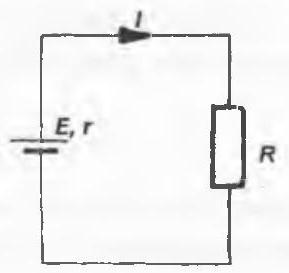
\includegraphics[max width=\textwidth]{2025_07_01_5b3ff9fa0d508c8e9f17g-353(2)}\\ Fig. prob. 3.62 \end{center}\\

3.63. Din Fig. prob. 3.63 b ): $I_{0}=\frac{E}{r+R}$ din care $r=\frac{E-I_{0} R}{I_{0}}$.\\ Din Fig. prob. 3.63 a) obținem: $I_{s}=\frac{2 E}{2 r+R}=\frac{2 I_{0} E}{2 E-I_{0} R}=4 \mathrm{~A}$.\\ \begin{center} 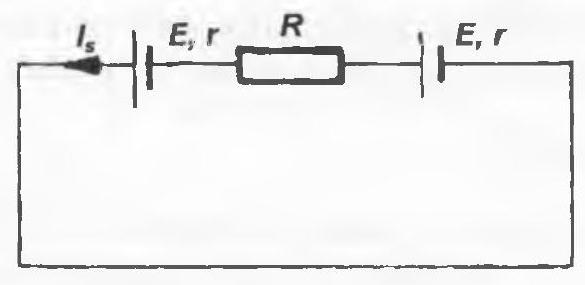
\includegraphics[max width=\textwidth, center]{2025_07_01_5b3ff9fa0d508c8e9f17g-353(1)}\\ Fig. prob. 3.63 a \end{center}\\ \begin{center} 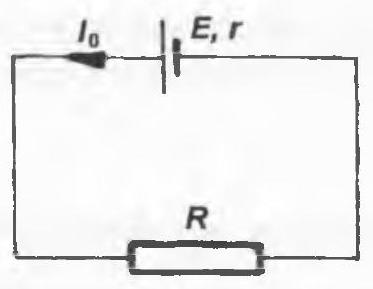
\includegraphics[max width=\textwidth, center]{2025_07_01_5b3ff9fa0d508c8e9f17g-353}\\ Fig. prob. 3.63 b \end{center}\\

3.64. $\Delta U=5 \%(220 \mathrm{~V})=11 \mathrm{~V}$, dar $\Delta U=R I=\rho \frac{l}{S} \cdot I \Rightarrow I=\frac{S \cdot \Delta U}{\rho \cdot l}=2,5 \mathrm{~A}$.\\

3.65. $I=\frac{N \cdot q}{t} \Rightarrow N=\frac{I \cdot t}{q}=1,2 \cdot 10^{20}$.\\

3.66. $W=E \cdot I \cdot t$ unde $E=\frac{\Delta \phi}{\Delta t}=S \cdot \frac{\Delta B}{\Delta t}=1,4 \cdot 10^{-3} \mathrm{~V}$.\\ $I=\frac{E}{R}=0,5 \mathrm{~A}$ şi $W=5,6 \cdot 10^{-4} \mathrm{~J}=560 \mu \mathrm{~J}$\\

3.67. $R_{t}=\frac{R_{1}}{2}+R_{2} ; I=\frac{E}{R_{t}}$. În acelaşi timp $I=\frac{E-U}{R_{2}}$. Din aceste relații:\\ $R_{2}=\frac{E-U}{U} \cdot \frac{R_{1}}{2}=1000 \Omega$\\

3.68. $E=I \cdot(R+r)$ de unde $r=\frac{E}{I}-R$. În cazul legării în serie:\\ $2 E=I_{s}(E+2 r) \Rightarrow I_{s}=\frac{2 E}{R+2 r}$\\ În cazul legării în paralel, din legea lui Kirchhoff:\\ Raportul,\\ $I_{p} R+\frac{I_{p} r}{2}=E \Rightarrow I_{p}=\frac{2 E}{2 R+r}$\\ $\frac{I_{s}}{I_{p}}=\frac{2 R+r}{R+2 r}=\frac{2 R+\frac{E}{I}-R}{R+2 \frac{E}{I}-R}=\frac{R+\frac{E}{I}}{2 \frac{E}{I}-R}=\frac{7}{5}$\\

3.69. Scriind legea lui Ohm pentru cele două situații:\\ $E=I_{1}\left(R_{1}+r\right) ; E=I_{2}\left(R_{2}+r\right)$ de unde $r=\frac{I_{2} R_{2}-I_{1} R_{1}}{I_{1}-I_{2}}=1 \Omega$ și $E=2 \mathrm{~V}$.\\ Pentru circuitul final: $I=\frac{E}{R_{1}+R_{2}+r}=\frac{2}{5} \mathrm{~A} ; P=U I=(E-I r) I=\frac{16}{25} \mathrm{~W}$.\\

3.70. Schema echivalentă a cablului scurtcircuitat este (Fig. prob. 3.70). Deoarece firele sunt identice, rezultă:\\ $R_{A}=R_{B}=\rho \frac{l_{1}}{S}$; \\ $R_{C}=R_{D}=\rho \frac{l_{2}}{S} ; l=A C=B D=l_{1}+l_{2}$\\ $R_{A B}=R_{A}+R_{B}=2 R_{A}$, de unde $R_{A}=15 \Omega$\\ $R_{C D}=R_{C}+R_{D}=2 R_{C}$, de unde $R_{C}=35 \Omega$\\ Din relațiile de mai sus,\\ $\frac{R_{A}}{R_{C}}=\frac{l_{1}}{l_{2}}$, adică $\frac{R_{A}}{R_{A}+R_{C}}=\frac{l_{1}}{l_{1}+l_{2}}$, iar $l_{1}=\frac{l R_{A}}{R_{A}+R_{C}}=1,5 \mathrm{~km}$\\ \begin{center} 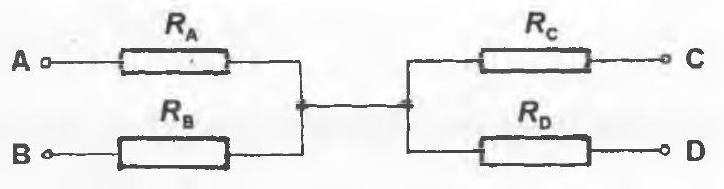
\includegraphics[max width=\textwidth]{2025_07_01_5b3ff9fa0d508c8e9f17g-354}\\ Fig. prob. 3.70 \end{center}\\

3.71. Aplicând legea a II-a a lui Kirchhoff buclei din stânga (Fig. prob. 3.71):\\ $I_{1} R_{1}=E_{1} \Rightarrow I_{1}=\frac{E_{1}}{R_{1}}=1 \mathrm{~A}$\\ Pentru bucla $B C D:-I_{2} R_{2}=-E_{2} \Rightarrow I_{2}=\frac{E_{2}}{R_{2}}=\frac{3}{4} \mathrm{~A}$.\\ În bucla $A C B:-I_{3} R_{3}+I_{2} R_{2}=-E_{1} \Rightarrow I_{3}=\frac{E_{1}+I_{2} R_{2}}{R_{3}}=4,5 \mathrm{~A}$.\\ Aplicând prima lege a lui Kirchhoff nodului $B, I_{2}+i_{1}=i_{2}+I_{1}$ şi nodului $A$,\\ $I_{1}+I_{3}=i_{3}$, adică $i_{3}=5,5 \mathrm{~A} \Rightarrow i_{4}=i_{1}-I_{1}+I_{2}$, de unde $I_{4}=5,25 \mathrm{~A}$.\\ \begin{center} 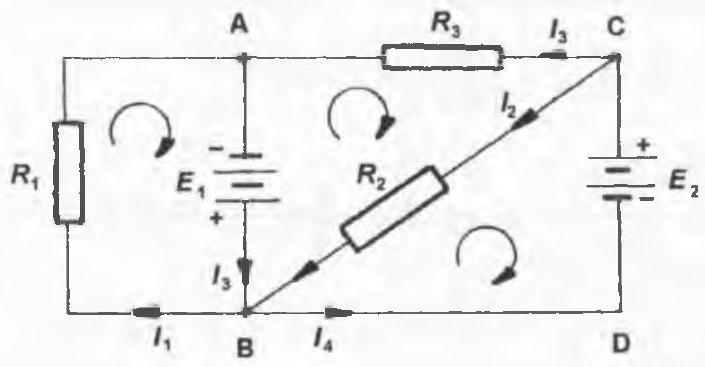
\includegraphics[max width=\textwidth, center]{2025_07_01_5b3ff9fa0d508c8e9f17g-355}\\ Fig. prob. 3.71 \end{center}\\

3.72. Puterea dată de sursă rezistorului are expresia $P=R I^{2}$, unde $I=\frac{E}{R+r}$, deci:\\ $P=\frac{R}{(r+R)^{2}} E^{\overline{2}}$\\ Din această relație se obţine ecuația $R^{2}+2\left(r-\frac{E^{2}}{2 P}\right) R+r^{2}=0$.\\ Este evident că există două valori ale rezistenței, care satisfac relația:\\ $\sqrt{R_{1} R_{2}}=r$.\\

3.73. Deoarece rezistenţa ampermetrului este nulă rezultă:\\ $U=U_{R}=U_{V}=I \frac{R R_{V}}{R+R_{V}} \Rightarrow R_{Y}=\frac{R U}{R I-U}$.\\

3.74. Coeficientul de temperatură este dat de relația de definiție $\alpha=\frac{R-R_{0}}{R_{0} \cdot t}$ unde $R_{0}$ şi $R$ sunt rezistenţele la $0^{\circ} \mathrm{C}$, respectiv la temperatura $t$. Folosind dependența rezistenței cu temperatura de forma: $R=\frac{\rho_{0} l(1+\alpha t)}{S}$, obținem pentru sistemul celor două fire legate în paralel: $\alpha_{\text {paralel }}=\frac{\rho_{01} \alpha_{2}+\rho_{02} \alpha_{1}}{\rho_{01}+\rho_{02}}$.\\

3.75. Randamentul circuitului simplu serie este $\eta=\frac{R}{R+r_{i}}$, unde $R$ este rezistența de sarcină iar $r_{i}$ este rezistența internă a bateriei. Folosind această relație scrisă pentru cazul celor două surse legate inițial în circuit serie simplu, obținem:\\ $r_{i 1}=\bar{R} \frac{1-\eta_{1}}{\eta_{1}} ; r_{i 2}=R \frac{1-\eta_{2}}{\eta_{2}}$\\ În general, randamentul se calculează cu relația:\\ $\eta=\frac{\sum_{k} R_{k} I_{k}^{2}}{\sum_{k} R_{k} I_{k}^{2}+\sum_{k} r_{i k} I_{k}^{2}}$\\ Să notăm cu $I_{1}, I_{2}$ şi $I$ curenții prin baterii la legarea în paralel, respectiv prin rezistența de sarcină $R$ menținută constantă. Ei pot fi aflați din ecuațiile Kirchhoff:\\ $I R+I_{1} r_{i 1}=E ; I R+I_{1} r_{i 2}=E ; I=I_{1}+I_{2}$\\ unde am folosit $E_{1}=E_{2}=E$. Introducând curenții determinați de mai sus, respectiv expresiile rezistențelor interne în expresia randamentului, obținem:\\ $\eta=\frac{\eta_{1}+\eta_{2}-2 \cdot \eta_{1} \cdot \eta_{2}}{1-\eta_{1} \cdot \eta_{2}}$\\ Cu $\eta_{1}<1 ; \eta_{2}<1$, se verifică imediat că avem $\eta>\eta_{1} ; \eta>\eta_{2}$.\\

3.76. Legea a 2-a a lui Kirchhoff scrisă pe tot circuitul oferă curentul din sistem: $I=\frac{E_{1}-E_{2}}{R_{1}+R_{2}+R_{3}}$. Aceeaşi lege scrisă pe ochiul $\mathrm{A}-\mathrm{B}-E_{1}-R_{1}$, conduce la $U_{\mathrm{AB}}=E_{1}-R_{1} \cdot I$. Obținem în final $U=6,43 \mathrm{~V}$.\\

3.77. Din relația de definiție, $F=e N_{A}$ reprezintă sarcina transportată pentru un mol de substanță. Pentru $3 \mathrm{~moli}$ vom avea $3 \mathrm{~F}$.\\

3.78. $1 \mathrm{~J}=1 \mathrm{~CV}$.\\

3.79. Puterea maximă se disipează pentru $R=r$. Atunci $I=\frac{E}{2 r}=30 \mathrm{~A}$.\\

3.80. $E=U_{1}+U_{2}+I r \quad ; \quad E=U_{2}^{\prime}+I^{\prime} r$.\\ Rezistența celui de-al doilea voltmetru este $R_{V_{2}}=\frac{U_{2}}{I}=\frac{U_{2}^{\prime}}{I^{\prime}}$ de unde $\frac{I}{I^{\prime}}=\frac{U_{2}}{U_{2}^{\prime}}$. Rezultă $E=U_{1}+U_{2}+\frac{I}{I^{\prime}}\left(E-U_{2}^{\prime}\right)=U_{1}+U_{2}+\frac{U_{2}}{U_{2}^{\prime}}\left(E-U_{2}^{\prime}\right)$.\\ $E=\frac{U_{1} U_{2}^{\prime}}{U_{2}^{\prime}-U_{2}}=20 \mathrm{~V}.$\\

3.81. Din $P=I^{2} R$ rezultă $I_{1}=\sqrt{\frac{P}{R_{1}}} ; I_{2}=\sqrt{\frac{P}{R_{2}}}$. Conform legii lui Ohm, $E=I_{1}\left(R_{1}+r\right)=I_{2}\left(R_{2}+r\right)$; astfel că $\frac{R_{1}+r}{\sqrt{R_{1}}}=\frac{R_{2}+r}{\sqrt{R_{2}}}$, de unde $r=\sqrt{R_{1} R_{2}}=10 \Omega$\\ şi $E=\sqrt{\frac{P}{R_{1}}}\left(R_{1}+r\right)=\sqrt{P}\left(\sqrt{R_{1}}+\sqrt{R_{1}}\right)=60 \Omega$.\\

3.82. $R_{S}=\frac{R_{A}}{n-1}=\frac{R_{A}}{\frac{I}{I_{A}}-1}=1,515 \mathrm{~A}$.\\

3.83. $P=P_{1}+P_{2}=2 P_{1}=\frac{4 \cdot U^{2}}{R}$, de unde $R=\frac{4 U^{2}}{P}$. Asemănător, $P^{\prime}=P_{1}^{\prime}+P_{2}^{\prime}=2 P_{1}=\frac{U^{2}}{R_{1}}+\frac{U^{2}}{R_{2}}$, de unde $R_{1} R_{2}=\frac{4 U^{4}}{P^{\prime} P}$. Astfel $R_{1}+R_{2}=\frac{4 U^{2}}{P}$, iar $R_{1}=10 \Omega$ şi $R_{2}=6 \Omega$ sau invers.\\

3.84. Din legile lui Kirchhoff (Fig. prob. 3.84), $I=I_{1}+I_{2} ; \quad E_{1}=I R$; $I R+r_{2} I_{2}=E_{2}$ şi pentru $I_{1}=0$ rezultă $I=I_{2}$. Atunci: $E_{2}=R I_{2}$ şi $I_{2}=\frac{E_{1}}{R}$. Deci $\left(R+r_{2}\right) I_{2}=E_{2}$, sau $\left(R+r_{2}\right) \frac{E_{1}}{R}=E_{2}$, de unde $E_{1}=\frac{R E_{2}}{R+r_{2}}=90 \mathrm{~V}$.\\ \begin{center} 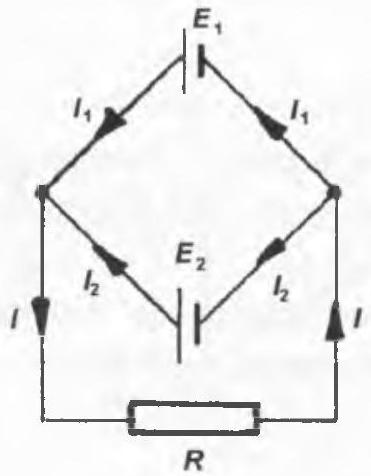
\includegraphics[max width=\textwidth, center]{2025_07_01_5b3ff9fa0d508c8e9f17g-357}\\ Fig. prob. 3.84 \end{center}\\

3.85. Rezistența echivalentă maximă se obține la legarea în serie, adică\\ $R_{s}=R_{1}+R_{2}+R_{3}=6 \Omega,$\\ iar rezistența echivalentă minimă la legarea în paralel, adică\\ $R_{p}=\frac{R_{1} R_{2} R_{3}}{R_{1} R_{2}+R_{2} R_{3}+R_{1} R_{3}}=\frac{6}{11} \Omega .$\\ Produsul cerut este: $p=R_{s} R_{p}=\frac{36}{11} \Omega^{2}$.\\

3.86. Randamentul \\ $\eta_{1}=\frac{R I}{E}=\frac{R}{E} \cdot \frac{E}{R+r}=\frac{R}{R+r}$, iar\\ $\eta_{2}=\frac{R}{E^{\prime}} \cdot \frac{E^{\prime}}{R+r^{\prime}}=\frac{R}{R+r^{\prime}}$\\ În cazul legării în serie, $\eta=\frac{R}{E+E^{\prime}} \cdot \frac{E+E^{\prime}}{R+r^{\prime}+R}$, deoarece $I=\frac{E+E^{\prime}}{R+r^{\prime}+R}$ şi atunci $\eta=\frac{R I I}{\left(E+E^{\prime}\right) I}=\frac{R}{E+E^{\prime}} \cdot \frac{E+E^{\prime}}{R+r^{\prime}+R}$, deci $R=\eta_{1} R+\eta_{1} r$, de unde\\ $r=\frac{R\left(1-\eta_{1}\right)}{\eta_{1}}=\frac{7}{3} R$\\ Dar, $r^{\prime}=R$ din $\left(\frac{1-0,5}{0,5}\right) R=r^{\prime}$. Rezultă $\eta=\frac{R}{\frac{7}{3} R+R+R}=0,23$.\\

3.87. Intensitatea de scurtcircuit este $I_{0}=\frac{E}{r}$, iar $I=\frac{E}{R+r}$, din legea lui Ohm. Randamentul $\eta=\frac{R I^{2}}{E I}=\frac{R I}{E}=\frac{R}{E} \cdot \frac{E}{R+r}=\frac{R}{R+r}$. Dar, $R+r=\frac{E}{I}$, iar $r=\frac{E}{I_{0}}$ şi atunci $R=E\left[\frac{1}{I}-\frac{1}{I_{0}}\right]$. Astfel, $\eta=I\left(\frac{1}{I}-\frac{1}{I_{0}}\right)=1-\frac{I}{I_{0}}=0,8$.\\

3.88. Rezistența grupării serie este $R=\frac{E}{I}=750 \Omega$. Deoarece rezistența echivalentă este $R=R_{1}+R_{2}+R_{3}$, se poate determina valoarea rezistenței necunoscute: $R_{3}=R-\left(R_{1}+R_{2}\right)=350 \Omega$.\\ Căderea de tensiune pe fiecare rezistor va fi:\\ $U_{1}=R_{1} I=8 \mathrm{~V} ; U_{12}=R_{2} I=4,8 \mathrm{~V} ; U_{3}=R_{3} I=11,2 \mathrm{~V}$\\ După cum se poate verifica: $U=U_{1}+U_{2}+U_{3}$.\\

3.89. Puterea disipată pe un rezistor $R$ pe care cade tensiunea electrică $U$ este: $P=\frac{U^{2}}{R}$. Deoarece se foloseşte aceeaşi sursă de energie singura mărime care se schimbă în cele două situații este rezistența.\\ Pentru gruparea serie: $R_{S}=R+R=2 R$, iar pentru gruparea paralel: $R_{p}=\frac{R \cdot R}{R+R}=\frac{R}{2}$. Ca urmare: $P_{s}=\frac{U^{2}}{2 R} ; P_{p}=\frac{U^{2}}{R / 2}$ de unde $\frac{P_{s}}{P_{p}}=\frac{1}{4}$.\\

3.90. Deoarece circuitul este format din două rezistoare grupate în serie, curentul electric care circulă prin circuit este același, egal cu $1 \mathrm{~A}$.\\

3.91. $P_{1}=\frac{U^{2}}{R_{1}} ; P_{2}=\frac{U^{2}}{R_{2}}$, de unde $R_{1}=\frac{U^{2}}{P_{1}} ; R_{2}=\frac{U^{2}}{P_{2}}$;\\ $R_{s}=R_{1}+R_{2}=R_{1}=\frac{U^{2}\left(P_{1}+P_{2}\right)}{P_{1} P_{2}} ; \frac{1}{R_{p}}=\frac{1}{R_{1}}+\frac{1}{R_{2}}=\frac{P_{1}+P_{2}}{U^{2}}$;\\ $P_{s}=\frac{U^{2}}{R_{s}}=\frac{P_{1} P_{2}}{P_{1}+P_{2}} ; P_{p}=\frac{U^{2}}{R_{p}}=P_{1}+P_{2}$\\ $\frac{W_{p}}{W_{s}}=\frac{P_{p} \tau}{P_{s} \tau}=\frac{\left(P_{1}+P_{2}\right)^{2}}{P_{1} P_{2}}=4,5$.\\

3.92. Pentru două rezistoare $R_{1}$ şi $R_{2}$ :\\ $R_{s}=R_{1}+R_{2} ; R_{p}=\frac{R_{1} R_{2}}{R_{1}+R_{2}} ; \quad \frac{R_{s}}{R_{p}}=\frac{\left(R_{1}+R_{2}\right)^{2}}{R_{1} R_{2}}>2^{2}$\\ Pentru trei rezistoare $R_{1}, R_{2}$ şi $R_{3}$ :\\ $R_{s}=R_{1}+R_{2}+R_{3} ; R_{p}=\frac{R_{1} R_{2} R_{3}}{R_{1} R_{2}+R_{2} R_{3}+R_{1} R_{3}}$\\ $\frac{R_{s}}{R_{p}}=\frac{\left(R_{1}+R_{2}+R_{3}\right)\left(R_{1} R_{2}+R_{2} R_{3}+R_{1} R_{3}\right)}{R_{1} R_{2} R_{3}}$

Ştiind că media aritmetică a trei numere diferite este mai mare decât media lor geometrică avem: $\frac{R_{1}+R_{2}+R_{3}}{3}>\sqrt[3]{R_{1} R_{2} R_{3}} ; \quad \frac{R_{1} R_{2}+R_{2} R_{3}+R_{1} R_{3}}{3}>\sqrt[3]{R_{1}^{2} R_{2}^{2} R_{3}^{2}}$, iar prin înmulțire: $\frac{\left(R_{1}+R_{2}+R_{3}\right)\left(R_{1} R_{2}+R_{2} R_{3}+R_{1} R_{3}\right)}{9}>R_{1} R_{2} R_{3}$, de unde $\frac{R_{s}}{R_{p}}>3^{2}$. Procedând la fel pentru $n$ rezistoare, $\frac{R_{S}}{R_{p}}>n^{2}$.\\

3.93. Din legea lui Ohm $I R+I r=E$ rezultă $R=\frac{E}{I}-r$. În al doilea caz, $n I \frac{R}{k}+n I r=E$. Înlocuind valoarea lui $R$ se obține relația $r I n\left(1-\frac{1}{k}\right)=E\left(1-\frac{n}{k}\right)$. Intensitatea curentului de scurtcircuit este $I_{0}=\frac{E}{r}=I \frac{n(k-1)}{k-n}$.\\

3.94. Cele două rezistențe legate în paralel pot fi înlocuite cu rezistența echivalentă $R_{p}=\frac{R_{3} R_{2}}{R_{3}+R_{2}}=\frac{12}{5} \Omega$. Astfel întregul circuit are rezistența echivalentă $R_{e}=R_{1}+R_{p}+R_{4}=4 \Omega$, iar $I=\frac{E}{R_{e}+r_{e}}==\frac{n e}{R_{e}+n r}=4 \mathrm{~A}$.\\

3.95. Din legea lui Ohm, $I_{1}=\frac{E}{R_{1}+r}$, iar $P_{1}=R_{1} I_{1}^{2}=\frac{R_{1} E^{2}}{\left(R_{1}+r\right)^{2}}$.\\ Asemǎnător, $I_{2}=\frac{E}{R_{2}+r}$ şi $P_{2}=R_{2} I_{2}^{2}=\frac{R_{2} E^{2}}{\left(R_{2}+r\right)^{2}}$. Din condiția $P_{1}=P_{2}$ rezultă $\sqrt{\frac{R_{1}}{R_{2}}}=\frac{R_{1}+r}{R_{2}+r}$, de unde $r=\sqrt{R_{1} \cdot R_{2}}$.\\

3.96. Legea lui Ohm pentru un circuit simplu este $I=\frac{E}{R+r}$, iar puterea disipată pe rezistenţa $R$ va fi: $P=R I^{2}=R \frac{E^{2}}{(R+r)^{2}}$ (1). Din enunțul problemei şi folosind relația (1) putem scrie: $P=R_{1} \frac{E^{2}}{\left(R_{1}+r\right)^{2}}=R_{2} \frac{E^{2}}{\left(R_{2}+r\right)^{2}}$ (2). Din relația (2) obținem: $\frac{R_{1}}{R_{2}}=\left(\frac{R_{1}+r}{R_{2}+r}\right)^{2}$ sau $\frac{\sqrt{R_{1}}}{\sqrt{R_{2}}}=\frac{R_{1}+r}{R_{2}+r}$. Din ultima relație rezultă: $r\left(\sqrt{R_{2}}-\sqrt{R_{1}}\right)=R_{2} \sqrt{R_{1}}-R_{1} \sqrt{R_{2}}$, de unde obținem: $r=\sqrt{R_{1} R_{2}}=10 \Omega \quad$ (3). Folosind prima parte a relației (2), datele din enunțul problemei şi relația (3) rezultă: $E=\left(R_{1}+r\right) \sqrt{\frac{P}{R_{1}}}=60 \mathrm{~V}$.\\

3.97. Intensitatea curentului prin circuit este: $I=\frac{U}{R_{V_{1}}+R_{V_{2}}}$, iar tensiunea indicată de fiecare voltmetru este:\\ respectiv\\ $U_{1}=I R_{1}=\frac{U}{R_{V_{1}}+R_{V_{2}}} R_{V_{1}}=10,9 \mathrm{~V}$, \\$ U_{2}=I R_{2}=\frac{U}{R_{V_{1}}+R_{V_{2}}} R_{V_{2}}=109,1 \mathrm{~V}$.\\

3.98. Rezistența echivalentă a rezistențelor grupate în paralel este: $R=\frac{R_{1} R_{2}}{R_{1}+R_{2}}=36 \Omega$. Intensitatea totală este: $I=\frac{U}{R}=3,33 \mathrm{~A}$. Intensitățile prin cele douǎ rezistenţe sunt: $I_{1}=\frac{U}{R_{1}}=2 \mathrm{~A}, I_{2}=\frac{U}{R_{21}}=1,33 \mathrm{~A}$ (la capetele fiecărui rezistor avem aceeaşi diferență de potențial de $120 \mathrm{~V}$).\\

3.99. Curentul care străbate circuitul este: $I=\frac{e-e^{\prime}}{R+r}=0,5 \mathrm{~A}$ unde $e$ este tensiunea electromotore a sursei, iar $e^{\prime}$ este tensiunea contraelectromotoare. Masa de argint care se depune în timpul procesului de electroliză este: $m=\frac{1}{F} \cdot \frac{A}{n} I t$, unde $F=96400 \mathrm{C} / \mathrm{Eg}, A$ masa atomică, iar $n$ valența. Înlocuind, se obține: $m=1 \mathrm{~g}$.\\

3.100 Rezistenta echivalentă a circuitului care este de forma: $R=\frac{R_{1} R_{2}}{R_{1}+R_{2}}$. Puterea absorbită de circuit este $P=R I^{2}=R\left(\frac{E}{R+r}\right)^{2}$. Puterea maximă se obține egalând derivata puterii în raport cu $R$ cu zero, adică: $\frac{d P}{d R}=0$ sau: $\frac{E^{2}(R-r)}{(R+r)^{2}}=0$, de unde se obține: $R=r$. Ţinând cont de expresia rezistenței $R$, se obține valoarea lui $R_{2}: R_{2}=\frac{r R_{1}}{R_{1}-r}=3 \Omega$.\\

3.101. Conform legii lui Joule-Lenz, $Q=U I t=U^{2} t / R$, de unde $R=U^{2} t / Q=9,97 \Omega \approx 10 \Omega$.\\

3.102. $V_{A}-V_{B}=E_{1}-E_{2}+I\left(R_{1}+R_{2}+r_{1}+r_{2}\right)=-11 \mathrm{~V}$.\\

3.103. Observăm că putem considera că rezistorul $R_{1}=7 R$ este în paralel cu $R$. Rezistența lor echivalentă este:\\ $I=E /\left(R_{\mathrm{ext}}+r\right)=10 E /(21 R)$, iar din legile Kirchhoff: \\ $I=I_{A}+I_{1}$ şi $I_{A} R=I_{1} R_{1} \Rightarrow I_{A}=I R_{1} /\left(R_{1}+R\right)=5 E /(12 R)$.\\

3.104. În lipsa şuntului, ampermetrul indică $N_{1}=50$ diviziuni pentru un curent $I_{1}=1 \mathrm{~A}$. Deci, valoarea unei diviziuni este $i_{0}=I_{1} / N_{1}=0,02 \mathrm{~A} / \mathrm{div}$.\\ În prezența şuntului, $I_{2}=5 \mathrm{~A}, N_{2}=10$, iar valoarea unei diviziuni este $i=\frac{I_{2}}{N_{2}}=0,5 \mathrm{~A} /$ div şi reprezintă factorul de mărire al scalei. Din formula rezistenței șuntului: $R_{S}=r /(n-1)=1,5 \Omega$.\\

3.105. Rezistențele $R_{V}$ şi $R / 3$ sunt legate în paralel (Fig. prob. 3.105). Rezistența lor echivalentă este: $R_{e}=R_{V} R /\left(3 R_{V}+R\right)$; intensitatea curentului principal:\\ $I=U /\left(R_{e}+2 R / 3\right)$\\ indicația voltmetrului este: $U_{V}=I R_{e}=96 \mathrm{~V}$.\\ \begin{center} 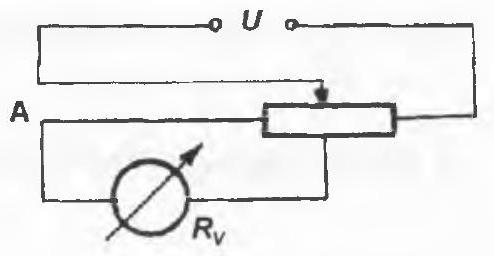
\includegraphics[max width=\textwidth]{2025_07_01_5b3ff9fa0d508c8e9f17g-362}\\ Fig. prob. 3.105 \end{center}\\


3.106. Puterea exterioară totală este egală cu suma puterilor din bec şi reostat: $P=U I+R I^{2}$; obținem ecuația: $I^{2}+I-20=0$ cu soluțiile: $I_{1}=4 \mathrm{~A}$ şi $I_{2}=-5 \mathrm{~A}$ (care nu are sens fizic); deci: $I=4 \mathrm{~A}$.\\

3.107. Pentru o sursă ideală $(r=0): P=E^{2} / R_{e} ; \quad P_{1} / P_{2}=R_{e 2} / R_{e 1}$; $R_{e 1}=5 R / 6 ; R_{e 2}=6 R$. Raportul $P_{1} / P_{2}=7,2$.\\

3.108. Cazul 1: $P=I_{1}^{2} R=\frac{E^{2} R}{(R+r)^{2}}$. Cazul 2: $R^{\prime}=1,8 R ; P^{\prime}=1,25 P$, dar: $P^{\prime}=\frac{E^{2} R^{\prime}}{\left(R^{\prime}+r\right)^{2}}$. Din aceste ecuații rezultă: $r=3 R$ şi $E^{2}=2400 R$. Cazul 3: $R^{\prime \prime}=0,75 R ; P^{\prime \prime}=\frac{E^{2} R^{\prime \prime}}{\left(R^{\prime \prime}+r\right)^{2}}=128 \mathrm{~W}$.\\

3.109. Randamentul circuitului: $\eta=\frac{P_{\text {utilā }}}{P_{\text {consumată }}}=\frac{I^{2} R}{I^{2}(R+r)}=\frac{R}{R+r}$; $\eta_{1}=\frac{R}{R+r_{1}}$ din care: $r_{1}=\frac{R\left(1-\eta_{1}\right)}{\eta_{1}}$. Analog: $r_{2}=\frac{R\left(1-\eta_{2}\right)}{\eta_{2}}$ şi $r_{\text {echiv }}=r_{1}+r_{2}=$ $=\frac{R(1-\eta)}{\eta}$; rezultă $\eta=\frac{\eta_{1} \eta_{2}}{\eta_{1}+\eta_{2}-\eta_{1} \eta_{2}} \cong 31,6 \%$.\\

3.110. $R^{\prime}=2 R / 3$ ( $R$ şi $2 R$ in paralel); $R^{\prime \prime}=R^{\prime}+R=5 R / 3$;\\ $1 / R_{\mathrm{e}}=1 / R^{\prime \prime}+1 / R^{\prime \prime}+1 / R=11 /(5 R) ; R_{\mathrm{e}}=10 \Omega ;$\\ Din legea lui Ohm pentru intregul circuit: $I=E /\left(R_{\mathrm{e}}+R_{\mathrm{V}}+r\right)=10 \mathrm{~A}$; din legea electrolizei: $m=k I t=10,8 \mathrm{~g}$.\\

3.111. $R_{\mathrm{e}}=4 R / 5$ şi intensitatea curentului principal este $I_{\mathrm{p}}=5 E /(4 R+5 r)$.\\

3.112. Intensitatea curentului este: $I=\frac{E}{R_{1}+R_{2}+r}=2 \mathrm{~A}$.\\

3.113. Conform Fig. prob. 3.113: $I=I_{1}+I_{2}=10,5 \mathrm{~A} ; U_{A B}=R_{A} I_{1}=0,5 \mathrm{~V}$, unde: $R=\rho \frac{l}{S}=5 \cdot 10^{-2} \Omega$. Deci, $I_{2}=\frac{U}{R}=10 \mathrm{~A}$.\\ \begin{center} 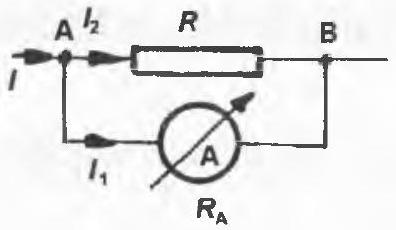
\includegraphics[max width=\textwidth, center]{2025_07_01_5b3ff9fa0d508c8e9f17g-363}\\ Fig. prob. 3.113 \end{center}\\

3.114. Conform Fig. prob. 3.114,\\ $I=\frac{E}{r+R}=12 \mathrm{~A} ; I_{1}=\frac{E}{r+1,5 R}=9 \mathrm{~A} ; \\ I_{2}=\frac{E}{r+0,75 R}=14,4 \mathrm{~A}$.\\ \begin{center} 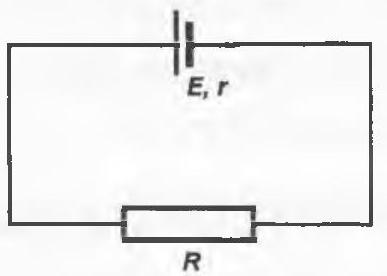
\includegraphics[max width=\textwidth, center]{2025_07_01_5b3ff9fa0d508c8e9f17g-363(1)}\\ Fig. prob. 3.114 \end{center}\\

3.115. Conform Fig. prob. 3.115,\\ $I=\frac{n E}{n r+\frac{R_{1} R_{2}}{R_{1}+R_{2}}}=12$, iar $\Delta U=I r=0,33 \mathrm{~V}$.\\ \begin{center} 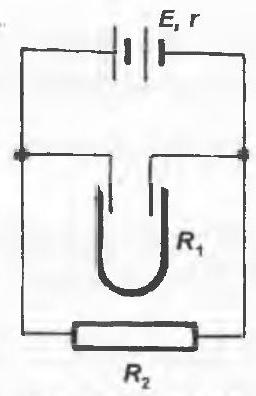
\includegraphics[max width=\textwidth, center]{2025_07_01_5b3ff9fa0d508c8e9f17g-364}\\ Fig. prob. 3.115 \end{center}\\

3.116. Din $j=\frac{I}{S}=n e v$ unde $I=\frac{q}{t}$ rezultă\\ $v=\frac{I}{S n e}=\frac{I}{\frac{\pi d^{2}}{4} n e}= 2,7 \cdot 10^{-6} \mathrm{~m} / \mathrm{s}$.\\ 

3.117 Conform Fig. prob. 3.117, $I = \frac{E}{r + R}$, $U_{AB}=I R=\frac{E}{r + R}$.\\ \begin{center} 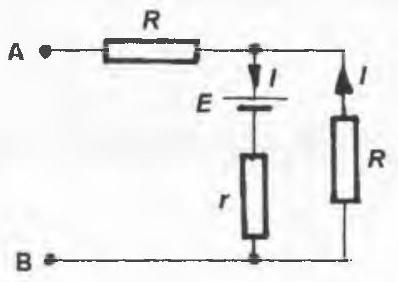
\includegraphics[max width=\textwidth, center]{2025_07_01_5b3ff9fa0d508c8e9f17g-364(1)}\\ Fig. prob. 3.117 \end{center}\\

3.118. $\phi=N_{1} B S=N_{1} \frac{\mu_{0} \mu_{r} N I}{l} \pi r^{2}=n^{2} l_{1} \mu_{0} \mu_{r} I \pi r^{2}=0,46 \mathrm{~Wb}$\\

3.119. Din $m \omega^{2} R=q v B=q \omega R B$, unde $\omega=\frac{q B}{m}=\frac{q \mu_{0} H_{0}}{m}$, rezultă $v=\frac{q B}{2 \pi m}=7,032 \cdot 10^{5} \mathrm{~s}^{-1}$.\\

3.120. Rezistența la $0^{\circ} \mathrm{C}$ este $R_{0}=\frac{120}{1,5}=80 \Omega$, iar rezistența la temperatura $t$ este $R=\frac{120}{1,33}=90 \Omega$. Pe de altă parte, expresia acesteia din urmă este: $R=R_{0}(1+\alpha t)$, de unde se poate calcula temperatura: $t=\frac{R-R_{0}}{R_{0} \alpha}=278^{\circ} \mathrm{C}$.\\

3.121. $B=\mu_{0} \mu_{r} \frac{N I}{l}=4,8 \cdot 10^{-4} \mathrm{~T}$.\\

3.122. Din legea inducției electromagnetice $e=-\frac{\Delta \Phi_{m}}{\Delta t}$ şi legea lui Ohm $I=\frac{e}{R}$ rezultă sarcina $q=I \Delta t=-\frac{\Delta \Phi_{m}}{R}=\frac{\Phi_{m_{\text {initial }}}-\Phi_{m_{\text { final }}}}{R}$, unde $\Phi_{m_{\text { initial }}}=\Phi$, iar $\Phi_{m_\text { final }}}=0$. Astfel, $q=\frac{\Phi}{R}=2 \cdot 10^{-4} \mathrm{~C}$.\\

3.123. Din condiția de mişcare pe cerc, $e v B=\frac{m v^{2}}{r}$, rezultă viteza:\\ $v=\frac{e}{m} B r=3,696 \cdot 10^{7} \mathrm{~m} / \mathrm{s}$\\

3.124. Din condiția de mişcare pe cerc, $\frac{m v^{2}}{r}=e v B$ rezultă:\\ $v=\frac{e}{m} r B=2,72 \cdot 10^{7} \mathrm{~m} / \mathrm{s}$\\

3.125. $\Phi=B N S=\mu_{0} \mu_{r} \frac{N I}{l} N S=\mu_{0} \frac{N^{2} I S}{l} ; n \Phi=\mu_{0} \mu_{r} \frac{N^{2}}{4} \frac{I}{4} \frac{S}{l}$;\\ $n=\frac{\mu_{r}}{16}=8$\\

3.126. Inducţia magnetică în centrul spirei trebuie să fie egală şi de sens opus inducţiei din solenoid:\\ $\mu \frac{I_{2}}{2 R}=\mu \frac{N I_{1}}{l} \Rightarrow I_{2}=N I_{1} \frac{2 R}{l}=10 \mathrm{~A}$.\\

3.127. Regula burghiului indică $\vec{B}$ perpendicular pe planul conductoarelor. Regula mâinii stângi indică forța electromagnetică în sensul BC.\\

3.128. Inducția generată de curentul $I_{1}$ este $B_{1}=\frac{\mu_{0} I_{1}}{2 \pi r}$, unde $r$ este distanța de la conductor la punctul considerat (Fig. prob. 3.128).\\ Forța de interacțiune culaturile buclei este:\\ $\vec{F}=I \vec{l} \times \vec{B}$\\ $\vec{F}_{3}$ şi $\vec{F}_{4}$ sunt egale şi de sens contrar, deci $\vec{R}_{34}=\vec{F}_{3}+\vec{F}_{4}=0$.\\ $F_{1}=I_{2} l \frac{\mu_{0} I_{1}}{2 \pi d} ; \quad F_{2}=I_{2} l \frac{\mu_{0} I_{1}}{2 \pi(d+L)}$\\ Rezultanta acestor două forțe va fi:\\ $R_{12}=F_{1}-F_{2}=\mu_{0} I_{1} I_{2} l\left(\frac{1}{d}-\frac{1}{d+l}\right)=7,2 \cdot 10^{-4} \mathrm{~N}$, şi este îndreptată spre fir.\\ \begin{center} 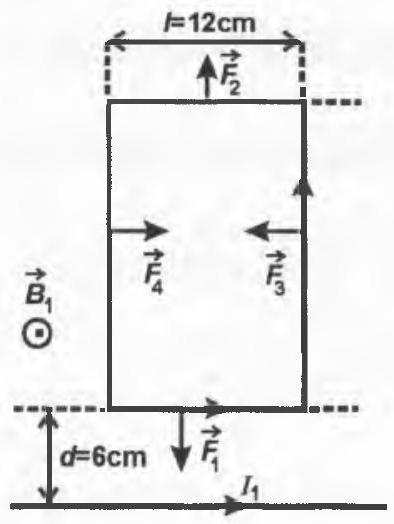
\includegraphics[max width=\textwidth, center]{2025_07_01_5b3ff9fa0d508c8e9f17g-365}\\ Fig. prob. 3.128 \end{center}\\

3.129. Semibucla de rază $R$ creează în centrul $O$ un câmp magnetic de inducţie $B_{1}=\frac{\mu_{0} I}{2(2 R)}$ (Fig. prob. 3.129), care intră în foaie.\\ Semibucla de rază $2 R$, creează un câmp de inducţie $B_{2}=\frac{\mu_{0} I}{2(2 \cdot 2 R)}=\frac{\mu_{0} I}{8 R}$, care iese din foaie. Inducția rezultantă va fi $B=B_{1}-B_{2}=\frac{\mu_{0} I}{8 R}$ şi va intra în foaie.\\ \begin{center} 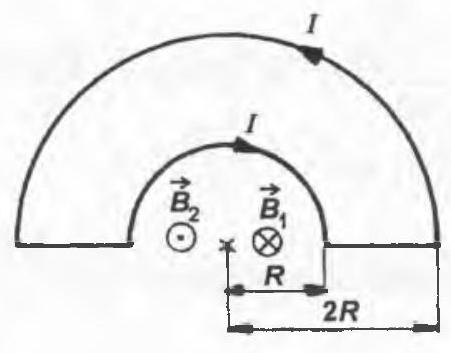
\includegraphics[max width=\textwidth, center]{2025_07_01_5b3ff9fa0d508c8e9f17g-366(1)}\\ Fig. prob. 3.129 \end{center}\\

3.130. Porțiunea AB din fir este în câmpul magnetic. Tensiunea din fir, $T$, este echilibrată de greutatea $G, T=G$ (Fig. prob. 3.130 a).\\ La echilibru, firul ia forma unui arc de cerc de rază $r$ şi în fiecare punct al arcului, rezultanta forțelor trebuie să fie zero.\\ Să considerăm o porțiune de arc de lungime (Fig. prob. 3.242 b) $\Delta l=r \Delta \theta$.\\ Asupra ei acționează:\\ \begin{itemize} \item forța electromagnetică, $F=B I \Delta l$; \item rezultanta tensiunilor de la capetele porțiunii \end{itemize}\\ $R=2 G \cos \left(\frac{\pi}{2}-\frac{\Delta \theta}{2}\right)=2 G \sin \frac{\Delta \theta}{2}$\\ Deci, la echilibru $B I \Delta l=2 G \sin \frac{\Delta \theta}{2}$, adică $B I r \Delta \theta=2 G \sin \frac{\Delta \theta}{2}$, sau $r=\frac{G}{B I} \frac{\sin \frac{\Delta \theta}{2}}{\frac{\Delta \theta}{2}}$.\\ Dar, în fiecare punct, $\Delta \theta \rightarrow 0$. Știind că $\lim _{\Delta \theta \rightarrow 0} \frac{\sin \frac{\Delta \theta}{2}}{\frac{\Delta \theta}{2}}=1$, se obține $r=\frac{G}{B I}$.\\ \begin{center} 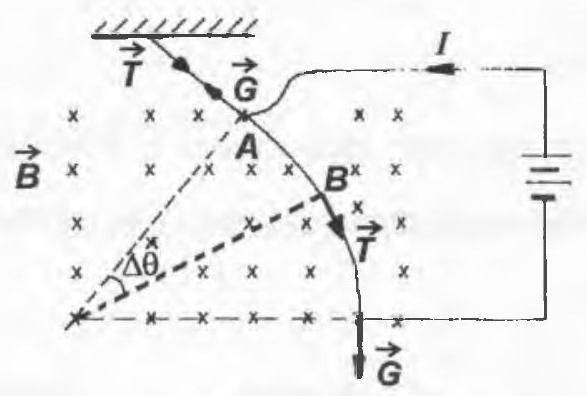
\includegraphics[max width=\textwidth, center]{2025_07_01_5b3ff9fa0d508c8e9f17g-366}\\ Fig. prob. 3.130.a \end{center}\\ \begin{center} 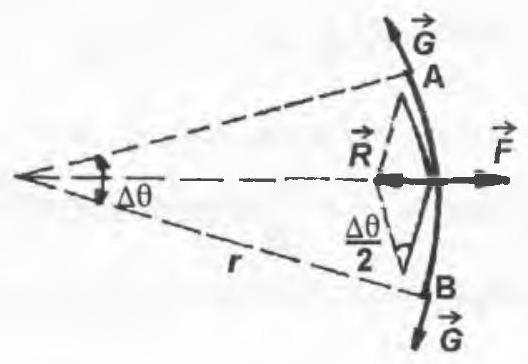
\includegraphics[max width=\textwidth, center]{2025_07_01_5b3ff9fa0d508c8e9f17g-366(2)}\\ Fig. prob. 3.130.b \end{center}\\

3.131. Viteza maximă se atinge când $F=B I l$, unde $B=\frac{\Phi}{S}$ şi $I=\frac{e}{R}=\frac{B l v}{R}$, astfel că: $v=\frac{F R S^{2}}{\Phi^{2} l^{2}}=0,8 \mathrm{~m} / \mathrm{s}$.\\

3.132. În timpul $t$ tija mătură unghiul la centru $\alpha=\omega t$ și suprafața $S=\frac{1}{2} r^{2} \omega t$. Fluxul magnetic care traversează aria spirei în intervalul de timp $t$ este: $\Phi=B S=\frac{1}{2} B r^{2} \omega t$, iar tensiunea electromotoare indusă,\\ $|e|=\frac{d \Phi}{d t}=\frac{1}{2} B \omega r^{2}=31,4 \mu \mathrm{~V}$\\

3.133. $t=\frac{T}{4}=\frac{1}{4} \cdot \frac{2 \pi R}{v}=\frac{\pi R}{2 v}=1,64 \cdot 10^{-3} \mathrm{~s}$.\\

3.134. Particula intră în zona cu câmp magnetic unde descrie o traiectorie circulară cu $R=\frac{m v}{q B}$. Pentru ca particula să nu atingă electrodul opus, este necesară condiția $R \leq d$. Obţinem in final $B=0,01 \mathrm{~T}$.\\

3.135. Considerăm o secțiune perpendiculară pe conductoare ca în Fig. prob. 3.135. Cu notațiile din figură, inducțiile magnetice create de curenții $I, 2 I$ în punctul unde se află conductorul parcurs de curentul $3 I$, vor avea modulele:\\ $B_{1}=\frac{\mu I}{2 \pi \sqrt{(d / 2)^{2}+x^{2}}} ; B_{2}=2 B_{1}$\\ Deoarece unghiul dintre cele două inducții este $2 \alpha$, rezultă inducţia totală în punctul în care se află conductorul $3 I$ :\\ $B(x)=\sqrt{B_{1}^{2}+B_{2}^{2}+2 B_{1} B_{2}\left(2 \frac{x^{2}}{(d / 2)^{2}+x^{2}}-1\right)}$ Inducția $B$ maximă este dată de ecuația $B^{\prime}(x)=0$; rezultă:\\ $x=\frac{d \sqrt{7}}{6} ; B_{\max }=\frac{9 I \mu}{4 \pi \sqrt{2} d}$\\ Forța pe unitatea de lungime căutată va fi $F_{\operatorname{maxim}}=3 I B_{\max }=\frac{27 \mu I^{2}}{4 \pi \sqrt{2} d}$.\\ \begin{center} 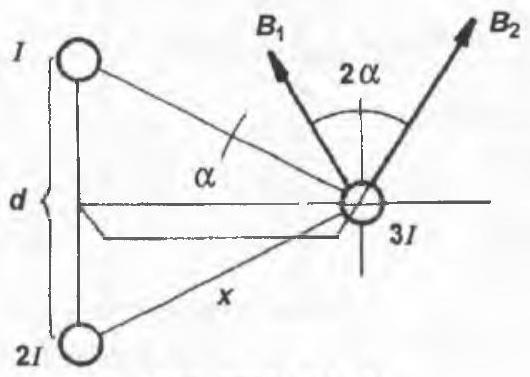
\includegraphics[max width=\textwidth, center]{2025_07_01_5b3ff9fa0d508c8e9f17g-367}\\ Fig. prob. 3.135 \end{center}\\

3.136. Deoarece unghiul dintre inducție şi normala la cadru este $\pi / 2$, rezultă că fluxul magnetic şi deci tensiunea indusă vor fí nule.\\

3.137. $B=B_{2}-B_{1}=\frac{\mu I_{2}}{\frac{2 \pi d}{2}}-\frac{\mu I_{1}}{\frac{2 \pi d}{2}}=\frac{\mu}{\pi d}\left(I_{2}-I_{1}\right)$, unde\\ $\frac{F}{l}=\frac{\mu I_{1} I_{2}}{2 \pi d} ; \quad \frac{\mu}{\pi d}=2 \frac{F}{l} \frac{1}{I_{1} I_{2}}$. Astfel, $B=2 \frac{F}{l} \frac{\left(I_{2}-I_{1}\right)}{I_{2} I_{1}}=0,5 \mathrm{~T} .$\\

3.138. $e=B l v=3 \mathrm{~V}$, iar $I=I_{1}+I_{2}$. Astfel $e=I r+I_{1} R_{1} ; I_{1} R_{1}=I_{2} R_{2}$, de unde $e=4 I_{1}+I_{2}, I_{1}=2 I_{2}$, adică $I_{1}=0,66 \mathrm{~A}, I_{2}=0,33 \mathrm{~A}$. Puterea $P=F v=B l I v=3 \mathrm{~W}$.\\

3.139. Din condiţia de mişeare pe cerc, $\frac{m v^{2}}{R}=q v B$ rezultã\\ $\frac{q}{m}=\frac{v}{R B}=4,8 \cdot 10^{7} \mathrm{C} / \mathrm{kg}$\\

3.140. Energia câmpului magnetic din solenoid este:\\ $W_{m}=\frac{L I^{2}}{2}=\mu_{0} \mu_{r} \frac{N^{2} S}{l} \cdot \frac{I^{2}}{2}$\\ După scoaterea miezului de fier energia devine: $W_{m}^{\prime}=\frac{L^{\prime} I^{2}}{2}=\mu_{0} \frac{N^{2} S}{l} \cdot \frac{I^{2}}{2}$, astfel că raportul $W_{m}^{\prime} / W_{m}=1 / \mu_{r}$. Deci energia scade de $\mu_{r}$ ori.\\

3.141. Fiind în vid, inducția magnetică în centrul spirei circulare este: $B=\mu_{0} \frac{I}{2 r_{0}}$. Pe de altǎ parte, $I=\frac{q}{T_{0}}=e \nu_{0}=e \frac{\omega_{0}}{2 \pi}=\frac{e}{2 \pi} \frac{v_{0}}{r_{0}}$. Rezultă\\ $B=\mu_{0} \frac{e v_{0}}{4 \pi r_{0}^{2}}$.\\

3.142. Punctul cel mai apropiat, la distantă egală de cele trei conductoare se află la intersecția mediatoarelor, deci la distanța $a$ de fiecare dintre conductoare. (Fig. prob. 3.142).\\ Astfel, $\left|\vec{B}_{1}\right|=\left|\vec{B}_{2}\right|=\left|\vec{B}_{3}\right|=\mu_{0} \frac{I_{1}}{2 \pi r}$, iar $a=\frac{2}{3} \sqrt{3 \frac{d^{2}}{4}}=\frac{d \sqrt{3}}{3}$ şi $\alpha=120^{\circ}$.\\ Deci $\vec{B}_{\text {rez }}=2 \vec{B}_{3}$ (deoarece $\vec{B}_{3}$ este pe direcția bisectoarei unghiului $\alpha$ ). În final, $\left|\vec{B}_{r e z}\right|=2 \mu_{0} \frac{3 I_{1}}{2 \pi d \sqrt{3}}=11,53 \cdot 10^{-6} \mathrm{~T}$.\\ \begin{center} 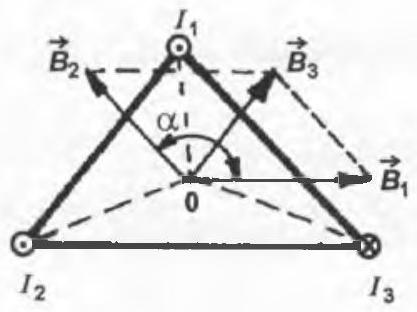
\includegraphics[max width=\textwidth, center]{2025_07_01_5b3ff9fa0d508c8e9f17g-369}\\ Fig. prob. 3.142 \end{center}\\

3.143. Variațiile fluxului magnetic la rotirea spirei este :\\ $\Delta \Phi=B S\left(\cos 0-\cos \frac{\pi}{6}\right)=\frac{\pi d^{2}}{4} B\left(1-\frac{\sqrt{3}}{2}\right)=0,134 \pi \frac{\pi d^{2}}{4} B$.\\ (Fig. prob. 3.143). Din legea Faraday, tensiunea electromotoare indusă este:\\ $e=\left|\frac{\Delta \Phi}{\Delta t}\right|$, iar din legea lui Ohm, $I=\frac{e}{R}$.\\ \begin{center} 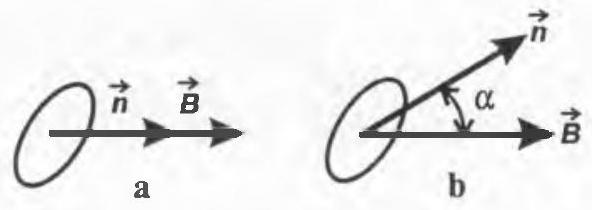
\includegraphics[max width=\textwidth, center]{2025_07_01_5b3ff9fa0d508c8e9f17g-369(1)}\\ Fig. prob. 3.143 \end{center}\\

Sarcina electrică indusă în spiră, $q=I \Delta t=\left|\frac{\Delta \Phi}{\Delta t}\right| \quad \frac{\Delta t}{R}=\frac{\Delta \Phi}{R} \quad q=1,077 \cdot 10^{-5} \mathrm{C}$.\\

3.144. Conform definiției, energia magnetică este $W=\frac{L I^{2}}{2}=\frac{\mu_{0} N^{2} S I^{2}}{2 l}$, unde $L=\frac{\mu_{0} N^{2} S}{l}$. În al doilea caz, $W^{\prime}=\frac{100 \mu_{0} N^{2} S I^{2}}{2 \cdot 2 l}$. Astfel, $\frac{W^{\prime}}{W}=50$.\\

3.145. Legea inducției electromagnetice se scrie (Fig. prob. 3.145):\\ $e=-B \frac{d S}{d t}$, unde $S=\frac{l}{2} \frac{x}{2}=x^{2} \operatorname{tg} \frac{\alpha}{2}$\\ Deci $e=B \cdot 2 x \frac{d x}{d t} \operatorname{tg} \frac{\alpha}{2}=2 B x v \operatorname{tg} \frac{\alpha}{2}$.\\ Intensitatea curentului,\\ $I=\frac{e}{R}=\frac{e}{r\left(2 x \operatorname{tg} \frac{\alpha}{2}+\frac{2 x}{\cos \frac{\alpha}{2}}\right)}=\frac{B v \sin \frac{\alpha}{2}}{r\left(1+\sin \frac{\alpha}{2}\right)}=25 \mathrm{~A} $.\\ \begin{center} 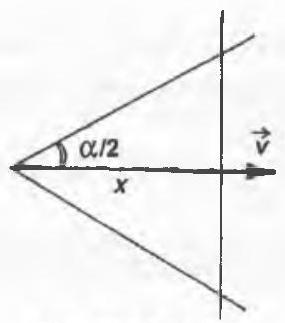
\includegraphics[max width=\textwidth]{2025_07_01_5b3ff9fa0d508c8e9f17g-370}\\ Fig. prob. 3.145 \end{center}\\

3.146. Forța Lorentz care acționează asupra particulei este de tip centripet. Ca urmare: $q v B=\frac{m v^{2}}{R}$, de unde $\omega=\frac{v}{R}=\frac{q B}{m}$. Dupã cum se observă frecvența de rotație nu depinde de viteza particulei şi deci nici de energia cinetică:\\ $v=\frac{\omega}{2 \pi}=\frac{q B}{2 \pi m}$\\

3.147. Tensiunea electromotoare indusă în spiră $|e|=\frac{\Delta \Phi}{\Delta t}=\frac{2 B S_{\text {spira }}}{\Delta t}$, cu $B=\mu \frac{N I}{l}$ şi $S_{\text {spira }}=\frac{\pi D^{2}}{4}(\Delta t-$ durata inversării sensului curentului $)$.\\ Curentul indus $i=\frac{|e|}{R}$ şi de pe altă parte $i=\frac{q}{\Delta t}$. Atunci\\ $q=i \Delta t=2 \frac{\mu N I}{e \Delta t} \cdot \frac{\pi D^{2}}{4} \Delta t=10^{-7} \mathrm{~C}$\\

3.148. Fluxul magnetic prin suprafaţa spirei nu variază, tensiunea indusă şi curentul indus sunt nule.\\

3.149. Din condiția de mişcare pe cerc, $\frac{m v^{2}}{R}=q v B$, rezultă :\\ $\frac{q}{m}=\frac{v}{R B}=2 \cdot 10^{7} \mathrm{C} / \mathrm{kg}$\\

3.150. Inducția câmpului magnetic, într-un punct aflat la distanța $r=\frac{a}{2}$ de conductor, este în valoare absolută: $B=\frac{\mu_{0} I}{2 \pi r}=\frac{\mu_{0} I}{2 \pi \frac{a}{2}}=\frac{\mu_{0} I}{\pi a}=1,2 \cdot 10^{-4} \mathrm{~T}$.\\ Dar, conform regulii, burghiului drept, inducția câmpului magnetic în punctul situat la mijlocul distanței dintre ei va fi: $B_{t}=2 B=2,4 \cdot 10^{-4} \mathrm{~T}$.\\

3.151. Pentru ca traiectoria particulei să fie circulară, trebuie ca forța Lorentz să fie egală cu forța centrifugă:\\ $\frac{m v^{2}}{R}=q v B$, de unde rezultă raza traiectoriei: $R_{1}=\frac{m v}{q B}$ (1)\\ În al doilea caz raza traiectoriei va fi: $R_{2}=\frac{m v}{2 q B}$ (2)\\ Împărțind relația (2) la relația (1) rezultă: $\frac{R_{2}}{R_{1}}=\frac{\frac{m v}{2 q B}}{\frac{m v}{q B}}=\frac{1}{2}$, din care obținem:\\ $R_{2}=\frac{R_{1}}{2}=2 \mathrm{~cm}$\\

3.152. Tensiunea electromotoare indusă care apare în conductor este (Fig. prob. 3.152): $e=B I v=12 \mathrm{~V}$. Dar conform regulii mâinii drepte, tensiunea $e$ dă naştere unui curent de sens contrar cu cel dat de sursă. Deci intensitatea curentului din circuit este: $I=\frac{E-e}{R+r}=4 \mathrm{~A}$.\\ \begin{center} 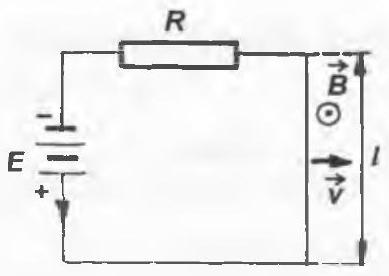
\includegraphics[max width=\textwidth, center]{2025_07_01_5b3ff9fa0d508c8e9f17g-371(1)}\\ Fig. prob. 3.152 \edn{center}\\

3.153. Avem: $F_{L}=B l l=B \frac{e}{R} l=B \frac{B l v_{l}}{R} l=\frac{B^{2} l^{2} v_{l}}{R}=m g$. Din ultima egalitate, $v_{l}=\frac{m g R}{B^{2} l^{2}}=10 \mathrm{~ms}^{-1}$.\\

3.154. Conform definiţiei, $B_{1}=\mu_{0} \frac{I_{1}}{2 \pi a}, \quad B_{2}=\mu_{0} \frac{I_{2}}{2 \pi a \sqrt{2}}=\mu_{0} \frac{\sqrt{2} I_{2}}{4 \pi a}$, $B_{3}=\mu_{0} \frac{I_{3}}{2 \pi a}$ (Fig. prob. 3.154).\\ Constatăm că, $B_{2}=\mu_{0} \frac{\sqrt{2} I_{2}}{4 \pi a}$, şi $B_{3}=\mu_{0} \frac{I_{1}}{2 \pi a}$.\\ Din figură observăm că:\\ $B^{2}=B_{1}^{2}+B_{2}^{2}+B_{3}^{2}=\frac{\mu_{0}^{2} I_{1}^{2}}{\pi^{2} a^{2}}$, de unde $B=\frac{\mu_{0} I_{1}}{\pi a}=2 \cdot 10^{-4} \mathrm{~Wb} \cdot \mathrm{~m}^{-2}$.\\ \begin{center} 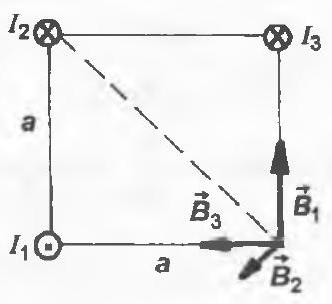
\includegraphics[max width=\textwidth, center]{2025_07_01_5b3ff9fa0d508c8e9f17g-371}\\ Fig. prob. 3.154 \end{center}\\

3.155. Condiția de stabilitate pe orbită este identificarea forței Lorentz cu forța centripetă: $\frac{m v^{2}}{r}=q v B$ adică $B=\frac{m v}{r q}$.\\ Fluxul magnetic ce străbate orbita va fi aşadar:\\ $\Phi=B \pi r^{2}=\frac{m v \pi r}{q}=2,14 \cdot 10^{-7} \mathrm{~Wb}$\\

3.156. Câmpul magnetic al curentului are valoarea $B=\frac{\mu_{0} I}{2 \pi d}$, find perpendicular pe direcţia curentului, deci şi pe cea a mişcǎrii electronului. Aşadar, forța de tip Lorentz exercitată de câmpul magnetic asupra electronului va avea valoarea:\\ $F=e v B=\frac{e v \mu_{0} I}{2 \pi d}=2,4 \cdot 10^{-20} \mathrm{~N}$\\ şi va fi îndreptată astfel încât să respingă electronul față de fir (situație analoagă celei a doi curenţi paraleli, dar de sens contrar).\\

3.157. Curenții fiind paraleli şi de acelaşi sens, se exercită atracție şi demonstrația nu poate reuşi - firul nu pluteşte.\\

3.158. Câmpul magnetic al curentului electric este $B_{i}=\frac{\mu I}{2 \pi r}=B_{e}$.\\ $r=\frac{\mu I}{2 \pi B_{e}}=\frac{4 \pi \cdot 10^{-7} \cdot 50}{2 \pi \cdot 10^{-3}}=10^{-2} \mathrm{~m}=1 \mathrm{~cm}$\\ Deoarece această relație este valabilă independent de $z$ rezultă o dreaptă paralelă cu conductorul, situată la $10 \mathrm{~mm}$ de acesta, într-un plan care cuprinde conductorul şi este perpendicular pe $\vec{B}$ (Fig. prob. 3.158).\\ \begin{center} 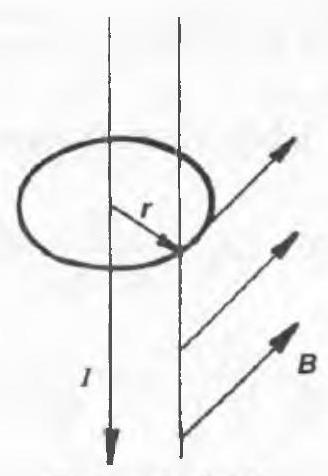
\includegraphics[max width=\textwidth, center]{2025_07_01_5b3ff9fa0d508c8e9f17g-372}\\ Fig. prob. 3.158 \end{center}\\

3.159. Din compunerea vectorilor $\vec{B}$ şi $\vec{B}_{0}$ rezultă că unghiul făcut de $\vec{B}_{r e z}$ cu direcția Nord este (Fig. prob. 3.159):\\ $\operatorname{arctctg} \frac{B_{0}}{B}=\alpha=\operatorname{arctctg} \frac{1}{\sqrt{3}}=\frac{\pi}{3}$.\\ \begin{center} 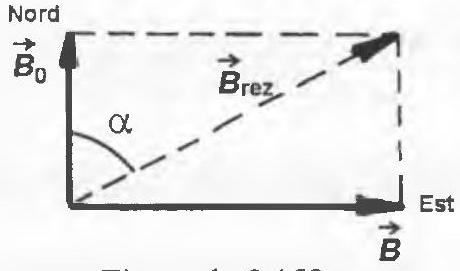
\includegraphics[max width=\textwidth, center]{2025_07_01_5b3ff9fa0d508c8e9f17g-373(1)}\\ Fig. prob. 3.159 \end{center}\\

3.160. $\vec{F}=I(\vec{l} \times \vec{B})=0$.\\

3.161. $L_{0}=\frac{\mu_{0} \mu_{r 0} N^{2} S}{l}=\mu_{0} n^{2} S l \mu_{r 0}$;\\ $L =\mu_{0} S n^{2}\left[p l \mu_{r 1}+(1-p) l \mu_{r 2}\right]= $\\$=\mu_{0} S n^{2} l\left[p \mu_{r 1}+(1-p) \mu_{r 2}\right]=L_{0}\left[p \mu_{r 1}+(1-p) \mu_{r 2}\right]=156 \mathrm{~N}$.\\

3.162. Răspuns corect: D).\\

3.163. Răspuns corect: D).\\

3.164. Răspuns corect: D ).\\

3.165. Fluxul magnetic apare in bobina prin care trece curentul $I_{b}=\frac{U}{R+R_{b}}$, $\operatorname{iar} \Phi=L I_{b}=\frac{U L}{R+R_{b}}=0,24 \mathrm{~mWb}$.\\

3.166. Aplicăm formula forței de interacțiune dintre doi curenți liniari, pe unitatea de lungime:\\ $F_{13} / l=\mu I_{1} I_{3} /(2 \pi a \sqrt{2})=\mu I^{2} \sqrt{2} /(2 \pi a)$\\$F_{23} / l=F_{43} / l=\mu I^{2} /(2 \pi a)$,\\ aceste forțe sunt perpendiculare (Fig. prob. 3.166). Obținem: $F_{3 \mathrm{rez}}=\sqrt{F_{13}^{2}+2 F_{23}^{2}}=\frac{\mu I^{2}}{\pi a}$\\ \begin{center} 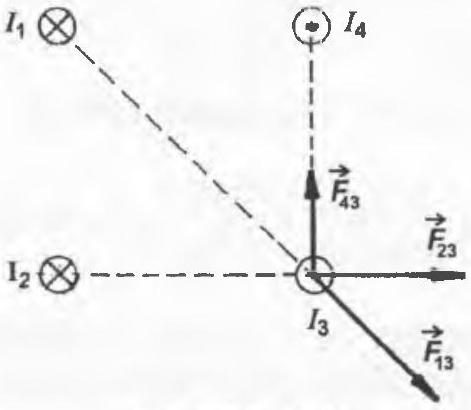
\includegraphics[max width=\textwidth, center]{2025_07_01_5b3ff9fa0d508c8e9f17g-373}\\ Fig. prob. 3.166 \end{center}\\

3.167. Forța Lorentz este forță centripetă:\\ $q v B=m v^{2} / r \Rightarrow v=q r B / m=101 \mathrm{~km} / \mathrm{s}$.\\

3.168. $n=N / l$; volumul, $V=S l$; inductanța, $L=\frac{\mu_{0} \mu_{r} N^{2} S}{l}=\mu_{0} \mu_{r} n^{2} V=$ $=15,2 \mathrm{~mH}$.\\

3.169. Inductanţa bobinei este: $L=\mu_{0} \mu_{r} n^{2} S l=6,4 \pi \mathrm{mH}$; din legea inducţiei electromagnetice, $e_{a}=-L \Delta I / \Delta t=L I / \Delta t=0,32 \pi \mathrm{~V}$.\\

3.170. Fluxul magnetic inițial: $\Phi_{i n}=B_{\nu} S \cos 0^{\circ}$; fluxul magnetic final: $\Phi_{\text {fin }}=B_{v} S \cos 180^{\circ} ; \Delta \Phi=2 B_{v} S$. Dar, $q=I \Delta t$, unde $I=e / R$, iar tensiunea electromotoare indusă este $e=-\frac{\Delta \Phi}{\Delta t}$. Astfel, sarcina electrică este egală cu $q=\frac{2 B_{v} a^{2}}{R}=0,5 \mu \mathrm{~C}$.\\

3.171. Numărul de rotații pe secundă (frecvența) are expresia $v=\frac{\omega}{2 \pi}=\frac{v}{2 \pi R}$, unde $v$ este viteza particulei, a cărei expresie rezultă din condiția de mişcare pe cerc a fiecărei particule în parte, adică $\frac{m v^{2}}{R}=q v B$, de unde $v=\frac{q B R}{m}$, cu $q$-sarcina particulei şi $m$-masa acesteia. Astfel, raportul căutat va fi:\\ $\frac{v_{e}}{v_{\alpha}}=\frac{\omega_{e}}{\omega_{\alpha}}=\frac{e}{m_{e}} \cdot \frac{m_{\alpha}}{2 e}=\frac{m_{\alpha}}{m_{e}}=3607,3$\\

3.172. Inducţia magnetică datorată primului strat este $B_{1}=\mu_{0} \frac{N_{1} I}{l}$, iar cea datorată celui de-al doilea strat este $B_{2}=\mu_{0} \frac{N_{2} I}{l}$. Inducţia magnetică totală va fi: $B=B_{1}+B_{2}=\mu_{0} \frac{I}{l}\left(N_{1}+N_{2}\right)=6,9 \cdot 10^{-3} \mathrm{~T}$.\\

3.173. Tensiunea electromotoare indusă în bobină este $e=-\frac{\Delta \Phi}{\Delta t}=$ $=-\frac{\left(\Phi_{f}-\Phi_{i}\right)}{\Delta t}=\frac{N B S \cos \alpha}{\Delta t}$, unde $\Phi_{f}$ este fluxul magnetic final care străbate bobina, iar $\Phi_{i}$ este fluxul magnetic inițial care străbate bobina. Curentul care străbate bobina este $i=\frac{e}{R}=\frac{N B S \cos \alpha}{R \Delta t}$. Dar, curentul prin definiție este $i=\frac{\Delta q}{\Delta t}$, unde $\Delta q$ este sarcina electrică. Egalând cele două relații pentru curent se obține:\\ $\Delta q=\frac{N B S \cos \alpha}{R}=2,4 \cdot 10^{-3} \mathrm{~C}$.\\

3.174. Tensiunea electromotoare indusă în spiră la întreruperea curentului prin electromagnet are expresia $e=-\frac{\Delta \Phi}{\Delta t}=-\frac{\Phi_{f}-\Phi_{i}}{\Delta t}$, unde $\Phi_{f}$ este fluxul magnetic final, egal cu zero, iar $\Phi_{i}$ este fluxul magnetic inițial, înainte de întreruperea alimentării, egal cu $\Phi$. Sarcina electrică totală care parcurge spira este: $q=i \Delta t=\frac{e}{R} \Delta t=\frac{\Phi}{R}$. Astfel, $\Phi=q R=10^{-4} \mathrm{~Wb}$.\\

3.175. Forța care acționează asupra inelului este $F=B i l$, iar forța pe unitatea de lungime este $f=\frac{F}{l}=B i$, unde $B$ este inducția magnetică din solenoid $B=\mu_{0} \frac{N I}{l}$, iar $i$ este intensitatea curentului indus $i=\frac{e}{R}$, unde $e$ este tensiunea electromotoare indusă:\\ $e=\frac{\mathrm{d} \phi}{\mathrm{~d} t}=\frac{\mathrm{d}}{\mathrm{~d} t}(B S)=\frac{\mathrm{d}}{\mathrm{~d} t}\left(\mu_{0} \frac{N I}{l} S\right)=\frac{\mathrm{d}}{\mathrm{~d} t}\left(\mu_{0} \frac{N k t}{l} S\right)=\frac{\mu_{0} N k S}{l}$.\\ Înlocuind se obține pentru intensitatea curentului indus expresia: $i=\frac{\mu_{0} N k S}{R l}$ şi $f=\frac{\mu_{0}^{2} N^{2} k^{2} S t}{R l^{2}}=28,4 \cdot 10^{-8} \mathrm{~N} / \mathrm{m}$.\\

3.176. Din condiția de echilibru (Fig. prob. 3.176) $F=G \Rightarrow B I l=m g$, unde $I=\frac{e}{R}=\frac{B l v}{R} \Rightarrow \frac{B^{2} l^{2} v}{R}=m g$, iar $v=\frac{m g R}{B^{2} l^{2}}=4 \mathrm{~m} / \mathrm{s}$.\\ \begin{center} 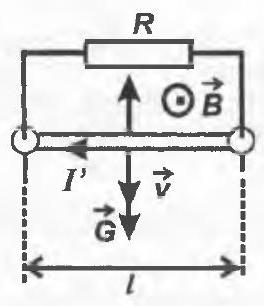
\includegraphics[max width=\textwidth, center]{2025_07_01_5b3ff9fa0d508c8e9f17g-375}\\ Fig. prob. 3.176 \end{center}\\

3.177. $e=B l v=B l \frac{m g}{M+m} t$, unde $v=a t=\frac{m g}{m+M} t$ (Fig. prob. 3.177). Deci $e=2 \mathrm{mV}$.\\ \begin{center} 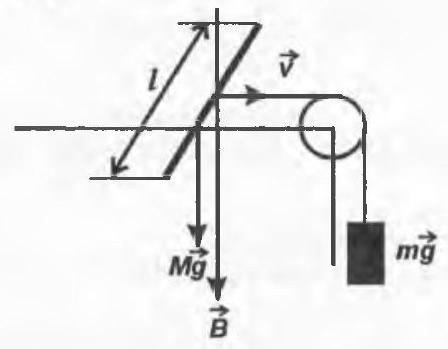
\includegraphics[max width=\textwidth, center]{2025_07_01_5b3ff9fa0d508c8e9f17g-375(1)}\\ Fig. prob. 3.177 \end{center}\\

3.178. Din condiția de egalitate a celor două forțe electrodinamice, $F_{13}=F_{23}$, adicã $\mu \frac{I_{1} I_{3} l}{2 \pi a}=\mu \frac{I_{2} I_{3} l}{2 \pi(d-a)} \Rightarrow d=\frac{a\left(I_{1}+I_{2}\right)}{I_{1}}=0,15 \mathrm{~m}$.\\

3.179. Tensiunile electromotoare induse în cele două spire sunt: $e_{1}=-\frac{\Delta \Phi}{\Delta t}=-S_{1} \frac{\Delta B}{\Delta t}$ şi $e_{2}=-S_{2} \frac{\Delta B}{\Delta t}$. Considerând $R$ rezistenţa firului, raportul curenților prin spire este: $\frac{I_{1}}{I_{2}}=\frac{e_{1} / R}{e_{2} / R}=\frac{S_{1}}{S_{2}}$, unde $S_{1}=\pi r^{2}=\pi\left(\frac{L}{2 \pi}\right)^{2}=\frac{L^{2}}{4 \pi}$ este suprafața spirei circulare, iar $S_{2}=\frac{L^{2} \sqrt{3}}{36}$ este suprafața triunghiului echilateral de perimetru $L$. Rezultǎ: $\frac{I_{1}}{I_{2}}=\frac{L^{2} / 4 \pi}{L^{2} \sqrt{3} / 36}=\frac{3 \sqrt{3}}{\pi}$.\\

3.180. Deoarece $\frac{m v^{2}}{q}=e U \Rightarrow m v^{2}=q e U$. Forța Lorentz este egală cu forta centrifugă: $F=\frac{m v^{2}}{r}=\frac{2 e U}{r}=1,28 \cdot 10^{-15} \mathrm{~N}$.\\

3.181. $B=\frac{\mu_{0} \mu_{r} N I}{l}=0,12 \pi \mathrm{~T}$.\\

3.182. Vectorial, $\vec{B}=\vec{B}_{1}+\vec{B}_{2}$, unde $B_{1}=\mu_{0} \frac{I_{1}}{2 \pi \frac{d}{2}} ; B_{2}=\mu_{0} \frac{I_{2}}{2 \pi \frac{d}{2}}$, iar scalar\\$B=B_{2}-B_{1}=\frac{\mu_{0}}{\pi d}\left(I_{2}-I_{1}\right)=10^{-5} \mathrm{~T}$\\

3.183. Se ține cont că $F=B I l \sin \alpha$; când conductorul este paralel cu liniile de câmp magnetic $\alpha=0$, deci $\sin \alpha=0$ și forţa este nulă, nu maximă. Corect $D$.\\

3.184. $B$ este inducția magnetică a unui câmp exterior în care este plasat conductorul, altul decât câmpul produs de curentul care trece prin conductor.\\

3.185. Forţa Lorentz este în permanență perpendiculară pe viteza de deplasare a particulei, deci accelerația tangențială este mereu nulă şi modulul vitezei rămâne în permanență acelaşi; în consecință, energia cinetică nu se modifică.\\

3.186. Inducţia electromagnetică înseamnă generarea tensiune electromotoare induse, care, în cazul de față, se datorează variației fluxului inducției magnetice şi are loc independent de proprietățile fizice locale ale mediului, putându-se produce inclusiv în vid. Spira nu are decât rolul de a pune în evidență existenţa unui curent electric indus.\\

3.187. Forţa Lorentz este în permanenţă perpendiculară pe viteza de deplasare a particulei, deci accelerația tangențială este mereu nulă și modulul vitezei rămâne în permanență acelaşi.\\

3.188. În ambele cazuri solenoizii $L_{\mathrm{A}}$ şi $L_{\mathrm{B}}$ sunt legați în serie, deci intensitatea curentului $I$ care trece prin ei este aceeaşi, atât în cazul din Fig. prob. 3.188.a, cât şi în cazul din Fig. prob. 3.188.b. În cazul a), ei nu se influentează unul pe celălalt, iar valoarea inducției magnetice pe axa fiecăruia este dată de $B=\mu_{0} \mu_{r} I \frac{N}{l}$, unde notațiile. În cazul b), câmpul pe axa comună este egală cu rezultatul superpoziției câmpurilor produse de cei doi solenoizi. Dacă solenoizii sunt bobinați în sensuri opuse, inducția magnetică produsă de fiecare dintre ei pe axa comună are sensuri contrare, conform cu regula mâinii drepte. Aşadar, inducția magnetică rezultantă este nulă.\\ \begin{center} 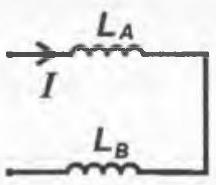
\includegraphics[max width=\textwidth, center]{2025_07_01_5b3ff9fa0d508c8e9f17g-377}\\ Fig. prob. 3.188 a \end{center}\\ \begin{center} 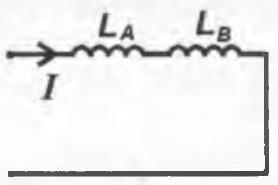
\includegraphics[max width=\textwidth, center]{2025_07_01_5b3ff9fa0d508c8e9f17g-377(1)}\\ Fig. prob. 3.188 b \end{center}\\

3.189. În ambele cazuri solenoizii $L_{\mathrm{A}}$ şi $L_{\mathrm{B}}$ sunt in serie, deci intensitatea curentului $I$ care trece prin ei este aceeaşi, atât în cazul a), cât şi în cazul b). În cazul a), ei nu se influențează unul pe celălalt, iar valoarea inducției magnetice pe axa fiecăruia este dată de $B=\mu_{0} \mu_{r} I \frac{N}{l}$, unde notațiile sunt cele cunoscute, şi este aceeaşi. În cazul b), câmpul pe axa comună este superpoziția câmpurilor produse de cei doi solenoizi. Dacă sensul de bobinaj al solenoizilor se păstrează acelaşi, inducția magnetică în punctul indicat nu se modifică, deoarece numărul de spire pe unitatea de lungime $\frac{N}{l}$ nu se modifică.\\

3.190. Mişcarea de translație în câmpul magnetic uniform nu produce flux magnetic variabil in circuitul electric delimitat de conturul spirei conductoare.\\

3.191. Sarcina $q=C U$, unde $U=S \frac{\Delta B}{\Delta t}=\pi R^{2} \frac{\Delta B}{\Delta t}$. Deci, $q=\pi R^{2} C \frac{\Delta B}{\Delta t}$.\\

3.192. Tensiunea electromotoare medie indusă este dată de:\\$e=-\frac{\Delta \Phi}{\Delta t}=\frac{N B S}{\Delta t}=6 \mathrm{~mV}$\\

3.193. Câmpul generat de solenoid este aproximativ uniform la mijlocul acestuia şi are valoarea $B=\frac{\mu_{0} N_{1} I_{1}}{L}$, iar în exteriorul solenoidului câmpul este nul. Fluxul prin a doua bobină va fi aşadar, $\Phi_{2}=N_{2} B \pi r^{2}=\frac{\mu_{0} N_{1} I_{1}}{L} N_{2} \pi r^{2}=M I_{1}$, de unde inductanța mutuală $M$ are expresia $M=\frac{\mu_{0} N_{1} N_{2} \pi r^{2}}{L}$.\\

3.194. $B_{1}=\mu_{0} \mu_{r} \frac{N I_{1}}{l} ; \Phi_{1}=B_{1} N S$;\\$B_{2}=\mu_{0} \mu_{r} \frac{N I_{2}}{l} ; \Phi_{2}=B_{2} N S$\\Întrucât $\Phi_{1}=\Phi_{2}$, rezultă: $B_{1}=B_{2}$ adică $I_{2}=2 I_{1}=4 \mathrm{~A}$, unde $N$ numărul de spire al fiecărei bobine, $S$ - secţiunea bobinei.\\

3.195. Tensiunea indusă va fi: $e=B l v$; rezultă prin rezistorul $R$ un curent:\\$i=\frac{e}{R}=\frac{B l v}{R}$, din care $B=\frac{I R}{l v}=2 \mathrm{~T}$\\

3.196. Dacă o bară de lungime $l$ se deplasează pe o distanţă $\Delta x$, într-un timp $\Delta t$, inducția magnetică fiind $B$, atunci variația fluxului magnetic are expresia: $\Delta \phi=B l \Delta x$. Conform legii inducţiei electromagnetice,\\$|e|=\frac{\Delta \phi}{\Delta t}=B l \frac{\Delta x}{\Delta t}=B l v=0,4 \mathrm{mV} .$\\

3.197. Forța Lorentz produce curbarea traiectoriei electronului şi este egală cu forta centrifugă, deci $e v B=\frac{m_{0} v^{2}}{R}$, iar $v=\sqrt{\frac{2 E_{c}}{m_{0}}}$, de unde\\$R=\frac{\sqrt{2 m_{0} E_{c}}}{e B}=10,7 \mathrm{~cm} ; T=\frac{2 \pi}{\omega}=\frac{2 \pi R}{\nu}=3,6 \cdot 10^{-7} \mathrm{~s}$\\

3.198. Răspuns corect: F).\\

3.199. Conform definiției, $F=B I l \sin \alpha$.\\ In primul caz: $\quad F_{1}=B I l \sin \frac{\pi}{2}=2 \cdot 10^{-2} \mathrm{~N}$.\\In al doilea caz: $\quad F_{2}=B I l \sin \frac{\pi}{3}=\sqrt{3} \cdot 10^{-2} \mathrm{~N}$.\\

3.200. Din legea inducţiei electromagnetice, $e=-\frac{\Delta \Phi}{\Delta t}=-\frac{\Phi_{f}-\Phi_{i}}{\Delta t}=\frac{B S}{2 \Delta t}$, unde $\Phi_{f}=B S \cos \left(\frac{\pi}{2}+30\right)=-B S \sin 30^{\circ}=-B S \frac{1}{2}$ şi $\Phi_{i}=0$.\\ Deci $\frac{e}{R}=i=\frac{q}{\Delta t}=\frac{B S}{2 R \Delta t}$, de unde $q=\frac{B S}{2 R}=4 \pi \mathrm{~mC}$.\\

3.201. Din legea inducţiei electromagnetice,\\$e=-N \frac{\Delta \Phi}{\Delta t}=-N \frac{\Phi_{f}-\Phi_{i}}{\Delta t}=-\frac{N\left(-\Phi_{i}\right)}{\Delta t}$, adică $e=-\frac{N \Phi}{\Delta t}$, de unde fluxul printr-o spiră $\Phi=\frac{e \Delta t}{N}=10^{-3} \mathrm{~Wb}$.\\

3.202. Din condiţia de mişcare pe cerc, $\frac{m v^{2}}{R}=2 e v B$, de unde:\\$m=\frac{2 e B R}{v}=2 \cdot 10^{-27} \mathrm{~kg} .$\\

3.203. $P=\frac{U^{2}}{R} \Rightarrow R=\frac{U^{2}}{P}=\frac{36}{2}=18 \Omega$\\$P=U I \Rightarrow I=\frac{P}{U}=\frac{2}{6}=\frac{1}{3} \mathrm{~A}$\\$E=I\left(R+R_{a}\right) \Rightarrow E=\frac{P}{U}\left(R+R_{a}\right) \Rightarrow R_{a}=\frac{U(E-U)}{P}=\frac{6(12-6)}{2}=18 \Omega$\\

3.204. $E=I_{1}\left(R_{1}+r\right) \Rightarrow r=\frac{E-I_{1} R_{1}}{I_{1}}$\\$E=I_{2}\left(R_{2}+r\right) \Leftrightarrow E-I_{2} R_{2}=\frac{I_{2}\left(E-I_{1} R_{1}\right)}{I_{1}} \Rightarrow$\\$E=\frac{I_{1} I_{2}\left(R_{2}-R_{1}\right)}{I_{1}-I_{2}}=\frac{0,8 \cdot 0,6(6-5)}{0,8-0,6}=2,4 \mathrm{~V}$\\

3.205. $B(t)=a+b t$\\ $e=\left|-\frac{\Delta \Phi}{\Delta t}\right|=\frac{S B(t)-S B\left(t_{0}\right)}{t-t_{0}}=\frac{S\left(a+b t-a-b t_{0}\right)}{t-t_{0}}=\frac{S b\left(t-t_{0}\right)}{t-t_{0}}=S b$\\

3.206. $P=R_{1} I_{1}^{2}=\frac{R_{1} E^{2}}{\left(r+R_{1}\right)^{2}}$\\ $P=R_{2} I_{2}^{2}=\frac{R_{2} E^{2}}{\left(r+R_{2}\right)^{2}}$\\ $\frac{R_{1} E^{2}}{\left(r+R_{1}\right)^{2}}=\frac{R_{2} E^{2}}{\left(r+R_{2}\right)^{2}} \Rightarrow r=\sqrt{R_{1} R_{2}}$\\ $I_{s c}=\frac{E}{r}=\frac{E}{\sqrt{R_{1} R_{2}}}$\\

3.207. $\eta=\frac{R}{R+r}$\\ $\begin{aligned}& I_{s}=\frac{E}{r} \Rightarrow r=\frac{E}{I_{s}}\\ & I=\frac{E}{R+r} \Rightarrow R+r=\frac{E}{I}\end{aligned}$\\ Tinând cont de ultimele două relații avem:\ $\eta=1-\frac{I}{I_{s}}$\\

3.208. $\overrightarrow{v_{y}} \perp \vec{B}, v_{y}=v \sin \alpha$\\ $\bar{R}=\frac{m v \sin \alpha}{q B}$\\

3.209. $U=R I$=$\frac{R E}{R+r} \Rightarrow R+r=\frac{R E}{U}$\\ $U^{\prime}=U(n+1)=\frac{4 R E}{4 R+r} \Rightarrow(n+1)=\frac{4 R E}{U(4 R+r)} \Rightarrow(n+1)=\frac{4 R E}{U[3 R+(R+r)]}$\\ $3 R(n+1)+(n+1)(R+r)=\frac{4 R E}{U}$\\ $3 R(n+1)+(n+1) \frac{R E}{U}=\frac{4 R E}{U} \Rightarrow E=\frac{3 U(n+1)}{3-n}$.\\

%% End %%